%==============================================================================
% Tento soubor použijte jako základ
% This file should be used as a base for the thesis
% Autoři / Authors: 2008 Michal Bidlo, 2022 Jaroslav Dytrych, 2025 Petr Veigend
% Kontakt pro dotazy a připomínky: sablona@fit.vutbr.cz
% Contact for questions and comments: sablona@fit.vutbr.cz
%==============================================================================
% kódování: UTF-8 (zmena prikazem iconv, recode nebo cstocs)
% encoding: UTF-8 (you can change it by command iconv, recode or cstocs)
%------------------------------------------------------------------------------
% zpracování / processing: make, make pdf, make clean
%==============================================================================
% Soubory, které je nutné upravit nebo smazat: / Files which have to be edited or deleted:
%   xkacha02-Large-models-math-20-literatura-bibliography.bib - literatura / bibliography
%   xkacha02-Large-models-math-01-kapitoly-chapters.tex - obsah práce / the thesis content
%   xkacha02-Large-models-math-01-kapitoly-chapters-en.tex - obsah práce v angličtině / the thesis content in English
%   xkacha02-Large-models-math-30-prilohy-appendices.tex - přílohy / appendices
%   xkacha02-Large-models-math-30-prilohy-appendices-en.tex - přílohy v angličtině / appendices in English
%==============================================================================
%\documentclass[english]{fitthesis} % bez zadání - pro začátek práce, aby nebyl problém s překladem
%\documentclass[english]{fitthesis} % without assignment - for the work start to avoid compilation problem
%\documentclass[zadani]{fitthesis} % odevzdani do IS VUT a/nebo tisk s barevnými odkazy - odkazy jsou barevné
\documentclass[english,zadani]{fitthesis} % for submission to the IS VUT and/or print with color links - links are color
%\documentclass[zadani,print]{fitthesis} % pro černobílý tisk - odkazy jsou černé
%\documentclass[english,zadani,print]{fitthesis} % for the black and white print - links are black
%\documentclass[zadani,cprint]{fitthesis} % pro barevný tisk - odkazy jsou černé, znak VUT barevný
%\documentclass[english,zadani,cprint]{fitthesis} % for the print - links are black, logo is color
\usepackage{xcolor}
\usepackage{tikz}
% * Je-li práce psaná v anglickém jazyce, je zapotřebí u třídy použít 
%   parametr english následovně:
%   If thesis is written in English, it is necessary to use 
%   parameter english as follows:
%      \documentclass[english]{fitthesis}
% * Je-li práce psaná ve slovenském jazyce, je zapotřebí u třídy použít 
%   parametr slovak následovně:
%   If the work is written in the Slovak language, it is necessary 
%   to use parameter slovak as follows:
%      \documentclass[slovak]{fitthesis}
% * Je-li práce psaná v anglickém jazyce se slovenským abstraktem apod., 
%   je zapotřebí u třídy použít parametry english a enslovak následovně:
%   If the work is written in English with the Slovak abstract, etc., 
%   it is necessary to use parameters english and enslovak as follows:
%      \documentclass[english,enslovak]{fitthesis}

% Základní balíčky jsou dole v souboru šablony fitthesis.cls
% Basic packages are at the bottom of template file fitthesis.cls
% zde můžeme vložit vlastní balíčky / you can place own packages here


% Pro seznam zkratek lze využít balíček Glossaries - nutno odkomentovat i níže a při kompilaci z konzoly i v Makefile (plnou verzi pro Perl, nebo lite)
% The Glossaries package can be used for the list of abbreviations - it is necessary to uncomment also below. When compiling from the console also in the Makefile (full version for Perl or lite)
%\usepackage{glossaries}
%\usepackage{glossary-superragged}
%\makeglossaries 

% Nastavení cesty k obrázkům
% Setting of a path to the pictures
%\graphicspath{{obrazky-figures/}{./obrazky-figures/}}
%\graphicspath{{obrazky-figures/}{../obrazky-figures/}}

%---rm---------------
\renewcommand{\rmdefault}{lmr}%zavede Latin Modern Roman jako rm / set Latin Modern Roman as rm
%---sf---------------
\renewcommand{\sfdefault}{qhv}%zavede TeX Gyre Heros jako sf
%---tt------------
\renewcommand{\ttdefault}{lmtt}% zavede Latin Modern tt jako tt

% vypne funkci šablony, která automaticky nahrazuje uvozovky,
% aby nebyly prováděny nevhodné náhrady v popisech API apod.
% disables function of the template which replaces quotation marks
% to avoid unnecessary replacements in the API descriptions etc.
\csdoublequotesoff

\usepackage{url}
\lstset{
    basicstyle=\ttfamily\small,
    backgroundcolor=\color{gray!10},
    frame=single,
    breaklines=true,
    columns=flexible,
    keepspaces=false
    }
% =======================================================================
% balíček "hyperref" vytváří klikací odkazy v pdf, pokud tedy použijeme pdflatex
% problém je, že balíček hyperref musí být uveden jako poslední, takže nemůže
% být v šabloně
% "hyperref" package create clickable links in pdf if you are using pdflatex.
% Problem is that this package have to be introduced as the last one so it 
% can not be placed in the template file.
\ifWis
\ifx\pdfoutput\undefined % nejedeme pod pdflatexem / we are not using pdflatex
\else
  \usepackage{color}
  \usepackage[unicode,colorlinks,hyperindex,plainpages=false,pdftex]{hyperref}
  \definecolor{hrcolor-ref}{RGB}{223,52,30}
  \definecolor{hrcolor-cite}{HTML}{2F8F00}
  \definecolor{hrcolor-urls}{HTML}{092EAB}
  \hypersetup{
	linkcolor=hrcolor-ref,
	citecolor=hrcolor-cite,
	filecolor=magenta,
	urlcolor=hrcolor-urls
  }
  \def\pdfBorderAttrs{/Border [0 0 0] }  % bez okrajů kolem odkazů / without margins around links
  \pdfcompresslevel=9
\fi
\else % pro tisk budou odkazy, na které se dá klikat, černé / for the print clickable links will be black
\ifx\pdfoutput\undefined % nejedeme pod pdflatexem / we are not using pdflatex
\else
  \usepackage{color}
  \usepackage[unicode,colorlinks,hyperindex,plainpages=false,pdftex,urlcolor=black,linkcolor=black,citecolor=black]{hyperref}
  \definecolor{links}{rgb}{0,0,0}
  \definecolor{anchors}{rgb}{0,0,0}
  \def\AnchorColor{anchors}
  \def\LinkColor{links}
  \def\pdfBorderAttrs{/Border [0 0 0] } % bez okrajů kolem odkazů / without margins around links
  \pdfcompresslevel=9
\fi
\fi
% Řešení problému, kdy klikací odkazy na obrázky vedou za obrázek
% This solves the problems with links which leads after the picture
\usepackage[all]{hypcap}


% Informace o práci/projektu / Information about the thesis
%---------------------------------------------------------------------------
\projectinfo{
  %Prace / Thesis
  project={BP},            %typ práce BP/SP/DP/DR  / thesis type (SP = term project)
  year={2026},             % rok odevzdání / year of submission
  date=\today,             % datum odevzdání / submission date
  %Nazev prace / thesis title
  title.cs={Velké jazykové modely pro řešení matematických úloh},  % název práce v češtině či slovenštině (dle zadání) / thesis title in czech language (according to assignment)
  title.en={Large language models for solving mathematical problems}, % název práce v angličtině / thesis title in english
  title.length={13.0cm}, % nastavení délky bloku s titulkem pro úpravu zalomení řádku (lze definovat zde nebo níže) / setting the length of a block with a thesis title for adjusting a line break (can be defined here or below)
  %sectitle.length={14.5cm}, % nastavení délky bloku s druhým titulkem pro úpravu zalomení řádku (lze definovat zde nebo níže) / setting the length of a block with a second thesis title for adjusting a line break (can be defined here or below)
  %dectitle.length={14.5cm}, % nastavení délky bloku s titulkem nad prohlášením pro úpravu zalomení řádku (lze definovat zde nebo níže) / setting the length of a block with a thesis title above declaration for adjusting a line break (can be defined here or below)
  %Autor / Author
  author.name={Rostyslav},   % jméno autora / author name
  author.surname={Kachan},   % příjmení autora / author surname 
  %author.title.p={Bc.}, % titul před jménem (nepovinné) / title before the name (optional)
  %author.title.a={Ph.D.}, % titul za jménem (nepovinné) / title after the name (optional)
  %Ustav / Department
  department={UPGM}, % doplňte příslušnou zkratku dle ústavu na zadání: UPSY/UIFS/UITS/UPGM / fill in appropriate abbreviation of the department according to assignment: UPSY/UIFS/UITS/UPGM
  % Školitel / supervisor
  supervisor.name={Martin},   % jméno školitele / supervisor name 
  supervisor.surname={Kostelník},   % příjmení školitele / supervisor surname
  supervisor.title.p={Ing.},   %titul před jménem (nepovinné) / title before the name (optional)
  %supervisor.title.a={},    %titul za jménem (nepovinné) / title after the name (optional)
  % Školitel specialista / Supervisor specialist
  % Vyplňuje se pouze u pojednání disertační práce nebo u disertační práce, pokud existuje školitel specialista. Pokud nemáte školitele specialistu, jméno a příjmení ponechte prázdné. / Is used only with PhD. thesis or proposal. if you have the specialist. If you do not have a specialist, leave name and surname blank.  
  specialist.name={},   % jméno školitele specialisty / supervisor specialist name 
  specialist.surname={},   % příjmení školitele specialisty / supervisor specialist surname
  specialist.title.p={},   %titul před jménem (nepovinné) / title before the name (optional)
  specialist.title.a={},    %titul za jménem (nepovinné) / title after the name (optional)
  % Klíčová slova / keywords
  keywords.cs={Velké jazykové modely, LLM, matematické uvažování, parametricky efektivní doladění, PEFT, Low-Rank Adaptation, LoRA, datová sada GSM8K, procesní model odměny, PRM, prohledávání hyperparametrů.}, % klíčová slova v českém či slovenském jazyce / keywords in czech or slovak language
  keywords.en={Large language models, LLM, mathematical reasoning, parameter-efficient fine-tuning,\\PEFT, Low-Rank Adaptation, LoRA, GSM8K dataset, process reward model, PRM, hyperparameter search.
 }, % klíčová slova v anglickém jazyce / keywords in english
  %keywords.en={Here, individual keywords separated by commas will be written in English.},
  % Abstrakt / Abstract
  abstract.cs={Tato práce se zabývá parametricky efektivním doladěním s cílem zlepšit matematické uva\-žování ve velkých jazykových modelech. Tři open-source modely s 7 miliardami parametrů --- Llama-2-7b-hf, Llama-2-7b-chat-hf a Mistral-7B-Instruct-v0.1 --- byly doladěny na datové sadě GSM8K pomocí Low-Rank Adaptation (LoRA), se systematickým prohledáváním rychlosti učení, LoRA ranku, alfy a efektivní velikosti dávky. Výkon byl hodnocen pomocí přesné shody a procesního modelu odměny Qwen2.5-Math-PRM-7B pro posouzení kvality dílčích kroků uvažování. Doladění přineslo podstatné zvýšení přesnosti: Llama-2-7b-hf se zlepšil z 10,77\% na 33,36\%, Llama-2-7b-chat-hf z 25,47\% na 39,88\% a Mistral-7B-Instruct-v0.1 z 42,23\% na 57,01\%. Výsledky ukazují, že LoRA s pečlivě vybranými hyperparametry účinně zlepšuje matematické uvažování, zatímco hodnocení PRM poskytuje další informace o kvalitě uvažování nad rámec pouhé přesnosti.
}, % abstrakt v českém či slovenském jazyce / abstract in czech or slovak language
  abstract.en={
  This thesis investigates parameter-efficient fine-tuning for improving mathematical reasoning in large language models. Three open-source 7-billion-parameter models --- Llama-2-7b-hf, Llama-2-7b-chat-hf, and Mistral-7B-Instruct-v0.1 --- were fine-tuned on the GSM8K dataset using Low-Rank Adaptation (LoRA), with a systematic search over learning rate, LoRA rank, alpha, and effective batch size. Performance was evaluated using exact-match accuracy and the Qwen2.5-Math-PRM-7B process reward model for assessing intermediate reasoning quality. Fine-tuning yielded substantial accuracy gains: Llama-2-7b-hf improved from 10.77\% to 33.36\%, Llama-2-7b-chat-hf from 25.47\% to 39.88\%, and Mistral-7B-Instruct-v0.1 from 42.23\% to 57.01\%. The results demonstrate that LoRA fine-tuning with carefully selected hyperparameters effectively enhances mathematical reasoning, while PRM evaluation provides additional insights into reasoning quality beyond accuracy alone.
}, % abstrakt v anglickém jazyce / abstract in english
  %abstract.en={An abstract of the work in English will be written in this paragraph.},
  % Prohlášení (u anglicky psané práce anglicky, u slovensky psané práce slovensky; u projektové praxe lze zakomentovat). Pokud použijete nástroje umělé inteligence, uveďte je podobně jako v příkladu. / Declaration (for thesis in english should be in english; for project practice can be commented out). If you use any AI tools, acknowledge them like in the provided example.
  declaration={I hereby declare that I have prepared this bachelor's thesis independently under the supervision of Ing. Martin Kostelník. All literary sources, publications, and other references used are listed in the bibliography. For the language revision of the technical report and rephrasing assistance, I used the tool Claude (Anthropic). For the development of the submitted program code, I also used the tool Claude (Anthropic).},
  %declaration={I hereby declare that this Bachelor's thesis was prepared as an original work by the author under the supervision of Mr. X
% The supplementary information was provided by Mr. Y
% I have listed all the literary sources, publications and other sources, which were used during the preparation of this thesis. I have used ChatGPT to correct spelling and other language mistakes. I used GitHub Copilot when working on the software. [specify and ammend based on reality].},
  % Poděkování (nepovinné, nejlépe v jazyce práce; nechcete-li, zakomentujte pro skrytí nadpisu. / Acknowledgement (optional, ideally in the language of the thesis; comment out to hide it including a heading.) 
  acknowledgment={I would like to thank my supervisor,
  Ing. Martin Kostelník, for his guidance, valuable feedback, and the time he devoted to assisting me with this bachelor's thesis.},
  %acknowledgment={Here it is possible to express thanks to the supervisor and to the people which provided professional help
%(external submitter, consultant, etc.).},
  % Rozšířený abstrakt (cca 3 normostrany) - lze definovat zde nebo níže / Extended abstract (approximately 3 standard pages) - can be defined here or below
  extendedabstract={Velké jazykové modely (LLM) dosáhly v posledních letech pozoruhodných výsledků v oblasti zpracování přirozeného jazyka, avšak matematické uvažování zůstává i pro výkonné modely náročnou oblastí. Modely trénované na různorodých textových korpusech z internetu sice disponují širokými jazykovými schopnostmi, ale nejsou specializované na strukturované víceúrovňové výpočty. Tato práce se zaměřuje na zlepšení matematického uvažování tří open-source modelů s 7 miliardami parametrů pomocí parametricky efektivního doladění metodou Low-Rank Adaptation (LoRA) na datové sadě GSM8K.

Pro experimenty byly vybrány tři modely představující odlišné typy předtrénování: Llama-2-7b-hf jako základní model bez instrukčního doladění, Llama-2-7b-chat-hf jako model doladěný pro dialogové účely pomocí metody supervised fine-tuning (SFT) a Reinforcement Learning from Human Feedback (RLHF), a Mistral-7B-Instruct-v0.1 jako instrukčně doladěný model, doladěný pouze pomocí SFT bez použití RLHF. Tato kombinace umožňuje zkoumat, jak typ předtrénování ovlivňuje optimální konfiguraci doladění a výslednou výkonnost.

Jako trénovací a evaluační datová sada byl zvolen GSM8K, který obsahuje 8 500 matematických slovních úloh na úrovni střední školy vytvořených lidskými autory. Každý příklad obsahuje otázku a postupné řešení zapsané v přirozeném jazyce --- tzv. chain-of-thought formát --- zakončené finální odpovědí označenou oddělovačem \#\#\#\#. Tento formát je výhodný zejména proto, že model musí při hledání odpovědi explicitně zaznamenat jednotlivé kroky uvažování, což podporuje strukturované matematické myšlení a zároveň umožňuje hodnotit kvalitu každého kroku samostatně pomocí procesního modelu odměny.

Doladění bylo provedeno prostřednictvím systematického prohledávání hyperparametrů rozděleného do čtyř sekvenčních experimentů. První experiment sloužil k nalezení referenční konfigurace kombinací rychlosti učení a LoRA ranku. Druhý experiment zkoumal vliv efektivní velikosti dávky na výkonnost. Třetí experiment analyzoval optimální rychlost učení pomocí jemnějšího rozlišení hodnot v okolí optima nalezeného v prvním experimentu. Čtvrtý experiment testoval různé kombinace ranku a parametru alfy. Každý model byl vyhodnocen na celé testovací sadě GSM8K.

Výkonnost modelů byla hodnocena dvěma metrikami. Primární metrikou byla přesnost (accuracy), definovaná jako podíl příkladů, u nichž model vygeneroval správnou číselnou odpověď. Sekundární metrikou bylo hodnocení pomocí procesního modelu odměny Qwen2.5-Math-PRM-7B, který přiřazuje skóre každému jednotlivému kroku uvažování a umožňuje tak posoudit kvalitu myšlenkového postupu nezávisle na finální odpovědi.

Doladění přineslo výrazné zlepšení přesnosti u všech tří modelů. Llama-2-7b-hf se zlepšil z výchozích 10,77 \% na 33,36 \%, Llama-2-7b-chat-hf z 25,47 \% na 39,88 \% a Mistral-7B-Instruct-v0.1 z 42,23 \% na 57,01 \%. Hodnocení PRM odhalilo, že doladění zlepšilo nejen přesnost, ale také kvalitu uvažování: modely přešly na strukturovaný formát odpovědí odpovídající trénovací datové sadě, a chybné odpovědi se staly lépe identifikovatelnými, protože obsahují jasně detekovatelný nesprávný krok.

Výsledky experimentů ukazují, že typ předtrénování silně ovlivňuje optimální konfiguraci doladění. Modely s vyšší výchozí výkonností vyžadují konzervativnější přístup s nižší rychlostí učení, zatímco základní modely potřebují agresivnější aktualizace. Kombinace přesnosti a PRM hodnocení poskytuje komplexnější pohled na schopnosti modelu než samotná přesnost.

Na závěr lze říci, že doladění pomocí LoRA s pečlivě nastavenými hyperparametry představuje efektivní přístup ke zlepšení matematického uvažování velkých jazykových modelů.},
  %extabstract.odd={true}, % Začít rozšířený abstrakt na liché stránce? / Should extended abstract start on the odd page?
  %faculty={FIT}, % FIT/FEKT/FSI/FA/FCH/FP/FAST/FAVU/USI/DEF
  faculty.cs={Fakulta informačních technologií}, % Fakulta v češtině - pro využití této položky výše zvolte fakultu DEF / Faculty in Czech - for use of this entry select DEF above
  faculty.en={Faculty of Information Technology}, % Fakulta v angličtině - pro využití této položky výše zvolte fakultu DEF / Faculty in English - for use of this entry select DEF above
  department.cs={Ústav matematiky}, % Ústav v češtině - pro využití této položky výše zvolte ústav DEF nebo jej zakomentujte / Department in Czech - for use of this entry select DEF above or comment it out
  department.en={Institute of Mathematics}, % Ústav v angličtině - pro využití této položky výše zvolte ústav DEF nebo jej zakomentujte / Department in English - for use of this entry select DEF above or comment it out
  tocdepth={1} % Nastavení zobrazení částí práce v obsahu (kapitoly, části, podčásti, atd.), 1 - zobrazují se nejvýše nadpisy první úrovně (kapitoly, části kapitol). Neměňte bez pokynu vedoucího. / Settings for what items are listed in the Table of contents. Default is 1 - just Chapters and Sections are listed. Do not change this setting without the direct order from the supervisor.
}

% Rozšířený abstrakt (cca 3 normostrany) - lze definovat zde nebo výše / Extended abstract (approximately 3 standard pages) - can be defined here or above
%\extendedabstract{Do tohoto odstavce bude zapsán výtah (abstrakt) práce v českém (slovenském) jazyce.}
% Začít rozšířený abstrakt na liché stránce? / Should extended abstract start on the odd page?
%\extabstractodd{true}

% nastavení délky bloku s titulkem pro úpravu zalomení řádku - lze definovat zde nebo výše / setting the length of a block with a thesis title for adjusting a line break - can be defined here or above
%\titlelength{14.5cm}
% nastavení délky bloku s druhým titulkem pro úpravu zalomení řádku - lze definovat zde nebo výše / setting the length of a block with a second thesis title for adjusting a line break - can be defined here or above
%\sectitlelength{14.5cm}
% nastavení délky bloku s titulkem nad prohlášením pro úpravu zalomení řádku - lze definovat zde nebo výše / setting the length of a block with a thesis title above declaration for adjusting a line break - can be defined here or above
%\dectitlelength{14.5cm}

% řeší první/poslední řádek odstavce na předchozí/následující stránce
% solves first/last row of the paragraph on the previous/next page
\clubpenalty=10000
\widowpenalty=10000

% checklist
\newlist{checklist}{itemize}{1}
\setlist[checklist]{label=$\square$}

% Kompilace po částech (rychlejší, ale v náhledu nemusí být vše aktuální)
% Compilation piecewise (faster, but not all parts in preview will be up-to-date)
% Další informace viz / For more information see https://www.overleaf.com/learn/latex/Multi-file_LaTeX_projects
% \usepackage{subfiles}

% Nechcete-li, aby se u oboustranného tisku roztahovaly mezery pro zaplnění stránky, odkomentujte následující řádek / If you do not want enlarged spacing for filling of the pages in case of duplex printing, uncomment the following line
% \raggedbottom

\begin{document}
  % Vysazeni titulnich stran / Typesetting of the title pages
  % ----------------------------------------------
  \maketitle
  % Obsah
  % ----------------------------------------------
  \setlength{\parskip}{0pt}

  {\hypersetup{hidelinks}\tableofcontents}
  
  % Seznam obrazku a tabulek (pokud prace obsahuje velke mnozstvi obrazku, tak se to hodi)
  % List of figures and list of tables (if the thesis contains a lot of pictures, it is good)
  \ifczech
    \renewcommand\listfigurename{Seznam obrázků}
  \fi
  \ifslovak
    \renewcommand\listfigurename{Zoznam obrázkov}
  \fi
  %{\hypersetup{hidelinks}\listoffigures}
  
  \ifczech
    \renewcommand\listtablename{Seznam tabulek}
  \fi
  \ifslovak
    \renewcommand\listtablename{Zoznam tabuliek}
  \fi
  % {\hypersetup{hidelinks}\listoftables}

  % Seznam zkratek / List of abbreviations
  %\ifczech
  %  \renewcommand*\glossaryname{Seznam zkratek}%
  %  \renewcommand*\entryname{Zkratka}
  %  \renewcommand*\descriptionname{Význam}
  %\fi
  %\ifslovak
  %  \renewcommand*\glossaryname{Zoznam skratiek}%
  %  \renewcommand*\entryname{Skratka}
  %  \renewcommand*\descriptionname{Význam}
  %\fi
  %\ifenglish
  %  \renewcommand*\glossaryname{List of abbreviations}%
  %  \renewcommand*\entryname{Abbreviation}
  %  \renewcommand*\descriptionname{Meaning}
  %\fi
  % Definice zkratek - z textu se odkazují např. \Gls{TF–IDF}
  % Definition of abbreviations - referred from the text e.g. \Gls{TF–IDF}
  %\newglossaryentry{TF–IDF}
  %{
  %  name={TF–IDF},
  %  description={Term Frequency-Inverse Document Frequency}
  %}
  % 
  %\setglossarystyle{superragged}
  %\printglossaries


  \ifODSAZ
    \setlength{\parskip}{0.5\bigskipamount}
  \else
    \setlength{\parskip}{0pt}
  \fi

  % vynechani stranky v oboustrannem rezimu
  % Skip the page in the two-sided mode
  \iftwoside
    \cleardoublepage
  \fi

  % Text prace / Thesis text
  % ----------------------------------------------
  \ifenglish
    % Author: Rostyslav Kachan

% For compilation piecewise (see projekt.tex), it is necessary to uncomment it and change
% \documentclass[../projekt.tex]{subfiles}
% \begin{document}
\chapter{Introduction}
\label{chap:introduction}
In an era where efficiency and automation are
  increasingly central to everyday work, large
  language models have emerged as powerful tools
  capable of assisting with a wide range of tasks
  --- from drafting emails and summarising documents  to translating text
  and generating code. Despite these impressive capabilities,
  mathematical reasoning remains a persistent
  challenge even for the most advanced models \cite{hendrycks2021}.
  This is a fundamental challenge rooted in how
  language models are built: they are trained on
  billions of words from books, articles,
  websites, and code --- a broad collection of
  general text that is not specifically focused
  on mathematical thinking.
  Unlike text generation or translation, solving
  mathematical word problems requires structured,
  multi-step reasoning where a single mistake
  can invalidate the entire solution. One
  practical path to closing this gap is
  fine-tuning --- adapting a pretrained model to a
  specific task using additional training data.
  However, fully retraining models with billions
  of parameters demands computational resources
  that are beyond the reach of most researchers.
  This thesis explores a more accessible
  alternative: Low-Rank Adaptation (LoRA) \cite{hu2022lora}, a
  parameter-efficient fine-tuning method that
  updates only a small fraction of model parameters
  while preserving the original weights.

  The goal of this thesis is to improve the
  mathematical reasoning capabilities of three
  open-source language models --- Llama-2-7b-hf \cite{touvron2023},
  Llama-2-7b-chat-hf \cite{touvron2023}, and Mistral-7B-Instruct-v0.1 \cite{jiang2023}
  --- through LoRA fine-tuning on the GSM8K \cite{cobbe2021}
  benchmark dataset. To find the most effective
  training configuration for each model, a
  systematic hyperparameter search was conducted
  across four experiments. In addition to
  accuracy, the quality of the models' reasoning
  steps was assessed using a process reward model,
  providing a deeper view of what fine-tuning
  actually changes in how the models think.

  My motivation for choosing this topic stems
  from a genuine interest in how large language
  models work and how they can be adapted for
  specific tasks. As these models become
  increasingly present in different fields such as customer
  service, healthcare, and software development,
  understanding the mechanisms behind their
  training felt both relevant and valuable.
  Mathematical reasoning was chosen as the focus
  because it offered a clear and measurable
  challenge: how much can fine-tuning actually
  improve a model's capabilities, and is that
  improvement visible beyond accuracy alone.

  The thesis is structured as follows.
  Chapter~\ref{chap:llms} introduces the
  theoretical foundations required to understand
  large language models and the methods used to
  adapt them for specific tasks.
  Chapter~\ref{chap:math-reasoning} covers
  state-of-the-art approaches to improving
  mathematical reasoning and the methods used
  to evaluate it. Chapter~\ref{chap:design}
  presents the design of the proposed solution.
  Chapter~\ref{chap:implementation} describes
  the most interesting aspects of the
  implementation. Chapter~\ref{chap:experiments}
  presents the experimental results and their
  discussion.
\chapter{Foundations of Large Language Models}
\label{chap:llms}

This chapter introduces the theoretical foundations required
to understand Large Language Models (LLMs) and the methods used
to adapt them for specific tasks. Fundamental concepts from Artificial Intelligence,
Machine Learning, and Neural Networks are presented, followed by  Language Modeling, the
Transformer architecture,
and the principles of LLMs.

\section{Artificial Intelligence and Machine Learning}
\label{sec:ai-ml}
The fundamental concepts of Artificial Intelligence and Machine
  Learning are introduced in this section, covering the principal
  AI research paradigms and the main Machine Learning approaches
  used in practice.

\subsection{Artificial Intelligence}

Artificial Intelligence (AI) is a field of computer
  science concerned with building intelligent entities
  --- machines capable of perceiving, reasoning, and
  acting effectively across a wide variety of tasks,
  from general problem-solving and learning to
  specialized applications such as proving mathematical
  theorems or diagnosing diseases \cite{russell2022}.

Historically, AI researchers have approached the definition of intelligence
along two dimensions: whether intelligence is measured against human
performance or rational behaviour, and whether the focus is on internal
thought processes or observable actions. This yields four
distinct research paradigms. The \textit{acting humanly} approach, represented
by the Turing Test, evaluates machine intelligence by whether a human
interrogator can distinguish a machine from a human through written
conversation. The \textit{thinking humanly} approach, rooted in cognitive
science, aims to build systems whose internal reasoning processes mirror those
of humans. The \textit{thinking rationally} approach attempts to formalise
correct reasoning through logic, extended by probability theory to handle
uncertain information. Finally, the \textit{acting rationally} approach defines
a rational agent as a system that acts so as to achieve the best outcome, or
when there is uncertainty, the best expected outcome.

The rational agent approach has prevailed throughout most of the field's
history, as it offers two key advantages over the alternatives. First, it is
more general than the laws of thought approach, since correct inference is
merely one of several mechanisms through which rationality can be achieved.
Second, the standard of rationality is mathematically well
  defined, which makes it possible to formally design agents
  that can be proven to achieve the specified goal --- something
  that is largely impossible when the goal is to imitate human
  behaviour, which lacks a precise formal definition. This paradigm
--- referred to as the standard model --- has influenced not only AI but also
control theory, operations research, and statistics. In practice, however,
perfect rationality is computationally infeasible in complex environments,
leading to the notion of \textit{limited rationality}, where agents act
appropriately under computational constraints.

\subsection{Machine Learning}
\label{subsec:ml}

Machine Learning (ML) is a subfield of Artificial Intelligence that enables
systems to learn from data and improve their performance without being
explicitly programmed.  It is
  particularly valuable in two situations: when designers cannot
  anticipate all possible future situations, or when the solution
  to a problem cannot be defined through explicit rules \cite{russell2022}. A program
  predicting stock market  \cite{chakravorty2025} illustrates the first
  case --- conditions change from boom to bust, making it
  impossible to define a fixed solution in advance. Face recognition \cite{sudiana2021}
  illustrates the second --- no programmer can explicitly define
  the rules that distinguish one face from another, yet the
  pattern can be learned from data. Machine learning algorithms
  are capable of solving both types of problems.

A formal definition of machine learning was introduced by Mitchell
\cite{mitchell1997}:

\begin{quote}
\textbf{Definition:} A computer program is said to \textbf{learn} from
experience $E$ with respect to some class of tasks $T$ and performance
measure $P$, if its performance at tasks in $T$, as measured by $P$,
improves with experience $E$.
\end{quote}

An illustrative example of this definition is a program
  that learns to play checkers.
The task $T$ is playing checkers games, the performance measure $P$ is the
percentage of games won against opponents, and the experience $E$ is obtained
by playing practice games against itself. As the program accumulates experience,
its performance at the task improves accordingly \cite{mitchell1997}. A
well-defined learning problem therefore requires three components: the class of
tasks, the performance measure, and the source of experience.

Machine learning encompasses a broad range of approaches, which differ
primarily in the type of feedback available during training. Among the
most commonly used paradigms are supervised learning, unsupervised
learning, reinforcement learning, and self-supervised learning.

\subsubsection*{Supervised Learning}

In supervised learning, the agent observes labeled input-output pairs
and learns a function that maps inputs to the correct outputs. The training
data acts as the teacher by providing correct labels, and the learned function
is subsequently used to predict outputs for previously unseen inputs.
A typical example is image classification, where a model is trained on images
labeled as ``bus'' or ``pedestrian'' and learns to correctly classify new
images \cite{russell2022}.

\subsubsection*{Unsupervised Learning}

Unsupervised learning, by contrast, requires no explicit feedback or
labels. Instead, the agent identifies patterns and structure directly in the
input data. The most common unsupervised task is \textit{clustering}, where similar
examples are grouped together based on shared characteristics. For instance,
when presented with millions of images from the Internet, a system can
automatically identify clusters of visually similar images --- such as those
that an English speaker would call ``cats'' --- without any prior labelling
\cite{russell2022}.

\subsubsection*{Reinforcement Learning}

A further paradigm is reinforcement learning, in which the agent
learns by interacting with an environment and receiving rewards
or punishments based on its actions. Rather than being provided with correct
answers, the agent must determine which of its actions were responsible for a
given outcome and adjust its behaviour accordingly to maximise future rewards.
A well-known example is a program learning to play chess: at the end of each
game, it receives a reward for winning or a punishment for losing, and over
time learns to improve its strategy \cite{russell2022}.


\subsubsection*{Self-Supervised Learning}

Self-supervised learning is a paradigm in which a system is
trained to capture the mutual dependencies between its inputs,
without requiring manually annotated labels \cite{lecun2022}.
Concretely, the model learns by predicting one part of the
input from another. A well-known example is BERT
  \cite{devlin2019}, which is pre-trained by randomly masking
  tokens in a sentence and learning to predict them from the
  surrounding context.

\section{Neural Networks and Deep Learning}

This section describes the difference between
  Neural Networks and Deep Neural Networks,
  followed by an introduction to Deep Learning.

\subsection{Neural Networks}
\label{sec:neural-networks}

A neural network is a computational model inspired by the structure of
biological neural networks found in the human brain \cite{nielsen2015,
goodfellow2016}. Neural networks are applied across a wide range of
tasks, including image recognition, natural language processing, and
speech recognition \cite{goodfellow2016}. The network is organised into layers of
artificial neurons: an input layer receives the raw
data, one or more hidden layers learn intermediate representations, and
an output layer produces the final result. The general structure of a
feedforward neural network is illustrated in
Figure~\ref{fig:nn-architecture}.

\begin{figure}[ht]
  \centering
  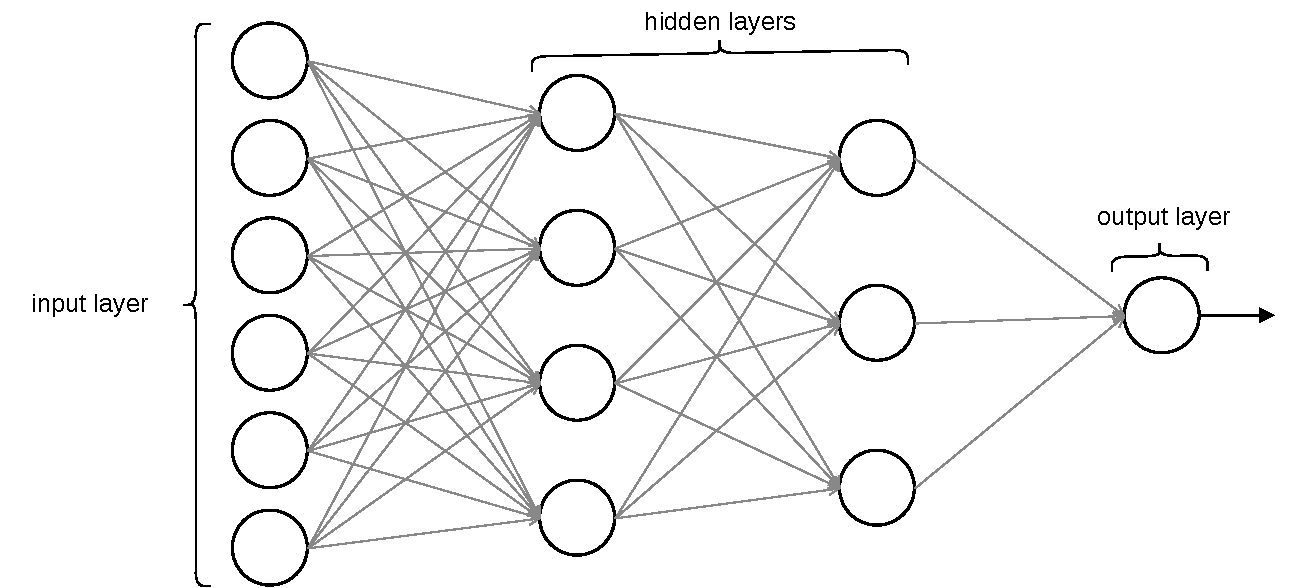
\includegraphics[width=0.8\textwidth]{figures/FINAL_NN.drawio.pdf}
  \caption{Architecture of a feedforward neural network.}
  \label{fig:nn-architecture}
\end{figure}



\subsection{Deep Neural Networks and Deep Learning}
\label{sec:deep-learning}

An artificial neural network with multiple hidden layers is called a
Deep Neural Network (DNN), and the practice of training such networks
is referred to as deep learning. The adjective \textit{deep} refers not
to the acquired knowledge, but to the number of layers that contribute
to the model \cite{montesinos2022}. Compared to conventional neural
  networks, deep neural networks employ more complex layer
  connections and a greater number of neurons, enabling them
  to capture non-linear aspects of complex data more
  effectively --- though at the cost of greater computational
  resources.

Image recognition serves as an illustrative example of
  deep learning in practice. Early layers of the network learn to detect
  simple low-level features such as edges and colour gradients.
  Deeper layers progressively combine these into more abstract
  representations --- shapes, textures, and eventually
  recognisable objects. This automatic construction of
  hierarchical representations from raw data is what enables
  deep networks to outperform shallower architectures on
  complex tasks, and forms the
  computational foundation upon which modern large language
  models are built.
\section{Language Modeling}
  \label{sec:language-modeling}

  A language model is a machine learning model that predicts
  upcoming words \cite{jurafsky2026}. More formally, it assigns
  a probability to each possible next word given the preceding
  context, or equivalently provides a probability distribution
  over possible next words. This can be expressed using the
  chain rule of probability, where the joint probability of a
  word sequence $w_1, w_2, \ldots, w_n$ is written as:
  \begin{equation}
    P(w_{1:n}) = \prod_{k=1}^{n} P(w_k \mid w_{1:k-1}),
    \label{eq:lm-compact}
    \end{equation}

    which expands to:

    \begin{equation}
    P(w_{1:n}) = P(w_1)\,P(w_2 \mid w_1)\,P(w_3 \mid w_{1:2})
    \cdots P(w_n \mid w_{1:n-1}).
    \label{eq:lm-expanded}
    \end{equation}

  Early approaches to language modeling relied on n-gram models
  --- the simplest kind of language model --- which estimate the
  probability of a word from a fixed window of previous words.
  The key insight underlying modern large language models is that
  training a model to predict upcoming words from large corpora
  enables it to learn an enormous amount about language. This objective, combined with the
  Transformer architecture described in the following section,
  forms the foundation of contemporary LLMs.

\section{Transformer Architecture}
\label{sec:transformer}
Prior to the Transformer, recurrent neural networks and their
variants --- Long Short-Term Memory and Gated Recurrent Units --- were
the dominant approaches to sequence modelling tasks such as language
modelling and machine translation. Recurrent models process input
sequentially, generating hidden states as a function of the previous
hidden state and the current input. This behaviour introduces significant limitations
during
  training: since each step depends on the previous one,
  parallelization is not possible, which becomes a major
  constraint for longer sequences \cite{vaswani2017}.

The Transformer, introduced by Vaswani et al. in 2017
  \cite{vaswani2017}, proposed a model architecture that
  dispenses with recurrence entirely, relying instead on an
  attention mechanism to capture dependencies between all
  positions in a sequence regardless of their distance. This allows for significantly more
  parallelization
compared to recurrent approaches.

\subsubsection*{Self-Attention}
The central mechanism of the Transformer is self-attention  \cite{vaswani2017}.
  For each position in the sequence, it computes a new
  representation by weighing contributions from all other
  positions, allowing the model to capture contextual
  information across the entire sequence. An attention function
  maps a query vector and a set of key-value vector pairs to
  an output, where the output is a weighted sum of the value
  vectors. The weight assigned to each value is determined by
  a compatibility function of the query with the corresponding
  key. In self-attention specifically, the
  query, key, and value vectors are all derived from the same
  input sequence. In mathematical notation, this is expressed
  as:

  \begin{equation}
  \text{Attention}(Q, K, V) = \text{softmax}
  \left(\frac{QK^T}{\sqrt{d_k}}\right)V,
  \label{eq:attention}
  \end{equation}

  where $Q$, $K$, and $V$ are the query, key, and value
  matrices respectively, and $d_k$ is the dimension of the
  keys and queries. Unlike recurrent models,
  self-attention allows each position in a sequence to attend
  to all other positions simultaneously, regardless of their
  distance.

\subsubsection*{Encoder-Decoder Architecture}

The Transformer follows an encoder-decoder structure, illustrated in
Figure~\ref{fig:transformer}. The encoder maps an input sequence of symbol representations
$(x_1, \ldots, x_n)$ to a sequence of continuous representations
$\mathbf{z} = (z_1, \ldots, z_n)$. Given $\mathbf{z}$, the decoder
generates an output sequence $(y_1, \ldots, y_m)$, consuming the previously generated
symbols as additional input
at each step. Both the encoder and decoder are composed of stacked layers containing
multi-head self-attention mechanisms and position-wise feed-forward
networks. In addition, the decoder inserts a third sub-layer, which
performs multi-head attention over the output of the encoder stack
\cite{vaswani2017}. While the original Transformer employs both encoder and decoder,
modern large language models typically adopt a decoder-only variant, relying solely on the
decoder stack to generate text autoregressively.

\begin{figure}[ht]
  \centering
  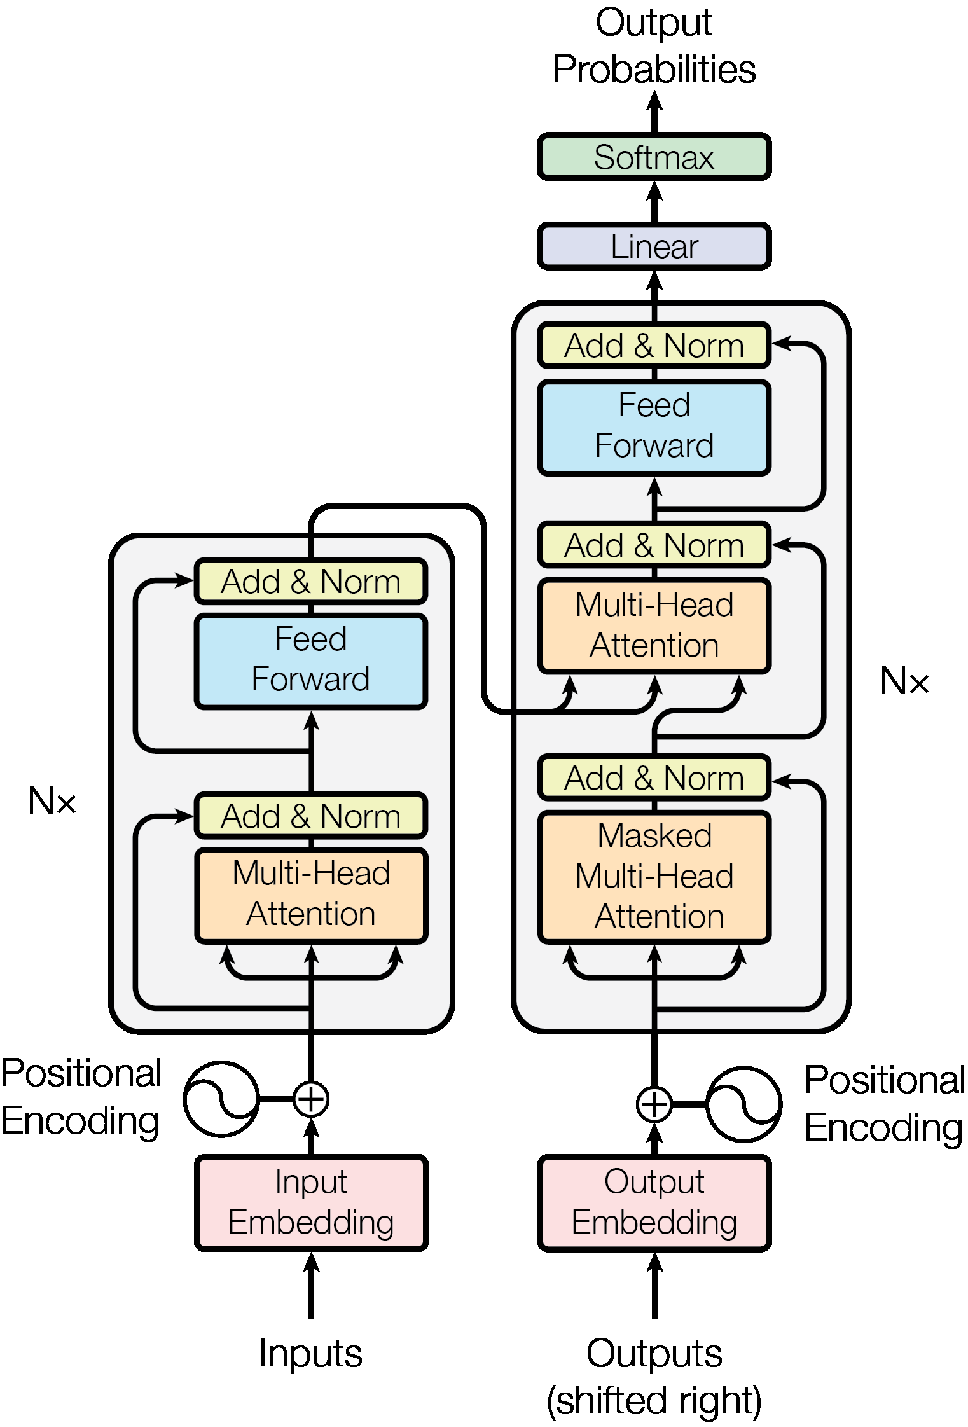
\includegraphics[width=0.45\textwidth]{figures/TEST_Transformer.drawio.pdf}
  \caption{The Transformer --- model architecture \cite{vaswani2017}.}
  \label{fig:transformer}
\end{figure}

\section{Large Language Models}
\label{sec:llms-detail}

Large Language Models (LLMs) are a category of language models
that utilise neural networks containing billions of parameters,
trained on enormous quantities of unlabelled text data using a
self-supervised learning approach \cite{raiaan2024}. Pre-trained
on large corpora from the web, these models learn complicated
patterns, language subtleties, and semantic linkages. LLMs have
demonstrated strong performance across a wide range of
language-related tasks, including text generation \cite{zhao2023survey}, translation
\cite{jiao2023chatgpt},
summarisation \cite{aly2025evaluation}, question answering \cite{singhal2025toward}, and
sentiment analysis
\cite{ghatora2024sentiment}.

The development of LLMs was enabled by three converging factors:
advances in deep learning, the availability of large-scale
computational resources, and access to vast quantities of
training data. Earlier approaches to language
modelling, such as statistical n-gram models and recurrent
neural networks, were limited by their inability to capture
long-term dependencies in text. The introduction of the Transformer architecture resolved these limitations by
enabling parallelisation and efficient modelling of long-range
dependencies, forming the architectural foundation of modern
LLMs.

\section{Fine-tuning}
\label{fine-tuning}

Fine-tuning is a process in which a pretrained model is
  adapted for particular tasks or domains by continuing to
  train the model using a domain-specific dataset that differs
  from the original pretraining data \cite{anisuzzaman2025}.
  Depending on the objective, fine-tuning can be used to teach
  the model to follow user instructions, to deepen its
  knowledge in a specific domain, or both. Various strategies
  exist for adjusting model parameters, ranging from updating
  all parameters to resource-efficient approaches that modify
  only a small subset. This section covers the distinction between base and
  instruction-tuned models, followed by the main fine-tuning
  strategies employed in practice: full fine-tuning, and
  parameter-efficient fine-tuning with its two widely adopted
  variants --- Low-Rank Adaptation (LoRA) \cite{hu2022lora} and its quantized
  counterpart QLoRA \cite{dettmers2023}.

\subsection{Instruction-Tuned vs.\ Base Models}
\label{sec:model-types}
A \textit{base model} is a large language model trained on
the objective of minimising contextual word prediction error
on large corpora of text. Through this process, the model
acquires broad language understanding and the ability to
generate coherent text. However, base models exhibit a
fundamental mismatch between their training objective and
the users' objective: while the model is optimised to
predict the next word in a sequence, users expect the model
to follow their instructions helpfully and safely
\cite{zhang2023}. As a result, base models often fail to
respond appropriately to explicit instructions, and may
produce outputs that are unhelpful, biased, or harmful.

To address this mismatch, \textit{instruction tuning} ---
also referred to as supervised fine-tuning (SFT) --- is
proposed as an effective technique to enhance the
capabilities and controllability of large language models
\cite{zhang2023}. It involves further training a base model on
  (instruction, output) pairs, where
  \textit{instruction} denotes a human instruction for the
  model and \textit{output} denotes the desired response. This process is illustrated
  in Figure~\ref{fig:instruct-tuning}. The benefits of instruction tuning are
threefold: it bridges the gap between the next-word
prediction objective and instruction following; it allows
for more controllable and predictable model behaviour; and
it is computationally efficient, enabling rapid adaptation
to specific domains without extensive retraining.

\begin{figure}[ht]
  \centering
  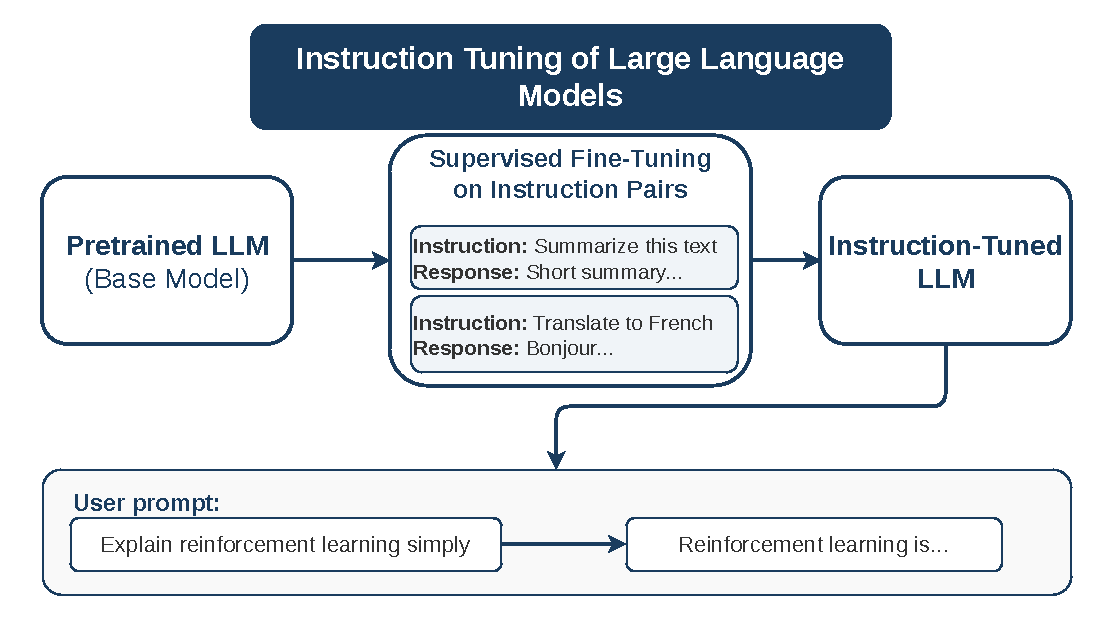
\includegraphics[width=0.8\textwidth]{figures/Instruction-Tune.pdf}
  \caption{{Illustration of instruction tuning: a pretrained base
  model is further trained on instruction-output pairs using
  supervised fine-tuning, producing an instruction-tuned model capable of
  following user instructions.}}
  \label{fig:instruct-tuning}
\end{figure}







\subsection{Full Fine-tuning}

Full fine-tuning updates all parameters of the pretrained
model during training, which typically yields strong
performance. However, as model scale increases --- reaching
175 billion trainable parameters in the case of GPT-3 ---
updating every parameter demands substantial computational resources,
  memory, and storage \cite{hu2022lora}, making it impractical for academic research
environments with limited hardware.

\subsection{Parameter-Efficient Fine-Tuning}

A widely adopted alternative, particularly when
computational resources are limited, is Parameter-Efficient
Fine-Tuning (PEFT) --- a technique in which a limited number
of model parameters are adjusted while keeping the remainder
unchanged \cite{han2024}. In practice, the original
pretrained weights are frozen, and only a small number of
newly introduced parameters are trained to adapt the model
to a specific task. Among the most widely adopted PEFT
methods are Low-Rank Adaptation (LoRA) and its quantized
variant QLoRA.

\subsection{Low-Rank Adaptation approach}


Low-Rank Adaptation (LoRA) \cite{hu2022lora} is a parameter-efficient fine-tuning
method that adapts pre-trained language models to downstream
tasks by introducing a small number of trainable parameters
while keeping the original model weights frozen.

The method is motivated by the finding that pre-trained
language models have a low intrinsic dimension \cite{aghajanyan2021} --- meaning
that despite having billions of parameters, the model's
behaviour can be effectively captured in a much smaller
subspace. In practice, when
  adapting a model to a new task, only a small fraction of
  its weights need to change to achieve good performance. LoRA exploits this by
  hypothesising that
the weight updates during adaptation also have a low
intrinsic rank \cite{hu2022lora}, and therefore can be represented compactly
using two small matrices instead of updating the full weight
matrix.

\subsubsection*{Low-Rank Parametrized Update Matrices}

The core concept of LoRA is illustrated  in Figure~\ref{fig:lora}. The
original pretrained weight matrix $W_0 \in \mathbb{R}^{d
\times k}$ is kept frozen during training and receives no
gradient updates. In parallel, two low-rank matrices are
introduced: matrix $A \in \mathbb{R}^{r \times k}$,
initialised with a random Gaussian distribution, and matrix
$B \in \mathbb{R}^{d \times r}$, initialised to zero,
ensuring that $\Delta W = BA$ has no effect at the beginning
of training \cite{hu2022lora}. The rank $r \ll \min(d, k)$
controls the size of these matrices and is significantly
smaller than the dimensions of the original weight matrix.

\begin{figure}[ht]
  \centering
  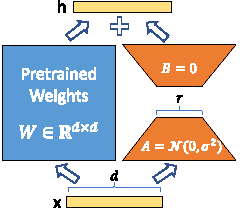
\includegraphics[width=0.35\textwidth]{figures/Lora_image.pdf}
  \caption{Illustration of LoRA approach: the frozen pretrained weight matrix $W_0$ is
  augmented by a low-rank decomposition $\Delta W = BA$, where
  $B$ is initialised to zero and $A$ with a random Gaussian
  distribution \cite{hu2022lora}.}
  \label{fig:lora}
\end{figure}

During the forward pass, the input $x$ is processed by both
the frozen path and the low-rank path simultaneously, and
their outputs are summed to produce the final output $h$:

\begin{equation}
  h = W_0 x + \Delta W x = W_0 x + BAx.
  \label{eq:lora}
\end{equation}

\subsubsection*{Hyperparameters}

The principal hyperparameter of LoRA is the rank  $r$ \cite{hu2022lora}, which
determines the size of the low-rank matrices $A$ and $B$
and consequently the number of trainable parameters. A lower
rank results in a more compact adaptation with fewer
parameters, while a higher rank allows more expressive
updates at the cost of increased memory usage.

The second hyperparameter is $\alpha$, a constant that
controls the magnitude of the LoRA update relative to the
rank. Together with $r$, it determines how strongly the
adaptation influences the pretrained model during
fine-tuning.

\subsubsection*{Advantages and Limitations}

LoRA offers several practical advantages over full fine-tuning \cite{hu2022lora}:

\begin{itemize}
  \item A pretrained model can be shared across multiple
  tasks by simply swapping the lightweight matrices $A$ and
  $B$, eliminating the need to store independent fine-tuned
  copies for each task.

  \item Training is more efficient as gradients and optimizer
  states are only computed for the small low-rank matrices
  rather than the entire model, lowering the hardware barrier
  to entry.

  \item When deployed, the matrices $A$ and $B$ can be merged
  with the frozen weights, introducing no additional inference
  latency compared to a fully fine-tuned model.

  \item LoRA is compatible with many prior fine-tuning methods and can be
  combined with them.
\end{itemize}

These benefits are reflected in concrete measurements on
GPT-3 175B: VRAM consumption during training is reduced
from 1.2TB to 350GB, checkpoint size decreases approximately
10{,}000 times from 350GB to 35MB with $r = 4$, and a 25\%
speedup during training is observed compared to full
fine-tuning \cite{hu2022lora}.

However, LoRA also has its limitations. When the matrices $A$ and $B$
are merged with the frozen weights to eliminate inference
latency, it is not straightforward to batch inputs from
different tasks in a single forward pass \cite{hu2022lora}.

\subsection{Quantized Low-Rank Adaptation approach}

Another widely used PEFT approach is Quantized Low-Rank
Adaptation (QLoRA)  \cite{dettmers2023}, which extends LoRA by first quantizing
the pretrained model weights to 4-bit precision and then
adding a small set of learnable low-rank adapter weights
that are tuned by backpropagating gradients through the
quantized weights. This is achieved
through two key innovations: 4-bit NormalFloat, an
information-theoretically optimal quantization data type
for normally distributed data that yields better empirical
results than standard 4-bit integers and floats; and Double
Quantization, a technique that quantizes the quantization
constants themselves, saving approximately 0.37 bits per
parameter. While QLoRA enables
fine-tuning of large models on hardware with significantly
limited VRAM, LoRA was employed in this thesis as it
operates on full-precision weights and therefore enables
more accurate parameter updates compared to QLoRA, where
quantization may introduce approximation errors during
adaptation.

\chapter{Mathematical Reasoning with Language Models}
\label{chap:math-reasoning}
This chapter presents an overview of current
  approaches to improving mathematical reasoning in
  large language models. It introduces chain-of-thought
  reasoning --- a technique that guides models to solve
  problems step by step --- along with its advantages
  and limitations. The chapter also presents process
  reward models as a method for evaluating the quality
  of intermediate reasoning steps produced by a model
  when solving mathematical problems.
\section{State of the Art}
\label{sec:sota}
Improving mathematical reasoning in large language models
  has attracted significant research attention. As models
  have grown in scale and capability, researchers have
  explored a range of strategies to close the gap between
  general-purpose LLMs and the level of mathematical
  proficiency required for reliable problem solving. Several
  approaches have emerged to address this challenge,
  including prompting-based methods \cite{wei2023}, supervised fine-tuning
  on mathematical data \cite{yu2024}, and process supervision
  \cite{lightman2024,qwen2025prm}, which are
  the most relevant to this work.

  \subsubsection*{Prompting-Based Approaches}

  One of the earliest and most influential directions is
  chain-of-thought (CoT) prompting, introduced by Wei et al.
  \cite{wei2023}, which improves reasoning by providing the
  model with a few step-by-step solution examples as part of
  the input prompt. Without any additional training, this
  approach raised the accuracy of PaLM 540B on the GSM8K
  benchmark from 17.9\% to 56.9\%. Kojima et al.
  \cite{kojima2022} further demonstrated that reasoning can
  be elicited even without any examples, simply by appending
  the phrase \textit{"Let's think step by step"} to each
  query --- a method referred to as zero-shot chain-of-thought
  prompting. This approach improved GSM8K accuracy from 10.4\% to
  40.7\% on InstructGPT (text-davinci-002) \cite{kojima2022}.
  However, these prompting approaches are most effective
  for very large models and provide limited gains for
  smaller open-source models, motivating the exploration
  of other approaches. Chain-of-thought reasoning is discussed in detail
  in Section~\ref{sec:cot}.

  \subsubsection*{Fine-Tuning on Mathematical Data}
  Another research direction focuses on supervised
  fine-tuning on domain-specific mathematical datasets.
  MetaMath \cite{yu2024} exemplifies this approach by
  augmenting existing math datasets through question
  bootstrapping --- rewriting questions using both forward
  and backward reasoning paths and rephrasing with LLMs
  --- creating a richer training set called MetaMathQA.
  Using LLaMA-2 as the base model, fine-tuning on
  MetaMathQA raises the accuracy of LLaMA-2 7B on GSM8K
  from 14.6\% to 66.5\%, outperforming the previous best
  open-source model of the same size by 11.5\%. This line
  of work demonstrates that targeted data augmentation
  combined with fine-tuning can substantially improve
  mathematical reasoning capabilities.

  \subsubsection*{Process Supervision}                                                   While fine-tuning approaches significantly improve
  accuracy on mathematical benchmarks, models can still
  arrive at correct answers through flawed intermediate
  reasoning steps --- a limitation that accuracy alone
  cannot detect. A further research direction therefore
  shifts focus from the final answer to the quality of
  each reasoning step. Two types of reward models have
  been proposed for this purpose: outcome reward models
  (ORMs), which evaluate only the final answer, and
  process reward models (PRMs), which assign a score to
  each individual reasoning step. In \textit{Let's Verify Step by Step}
  \cite{lightman2024},
  the authors compare outcome and process supervision,
  demonstrating that process supervision significantly
  outperforms outcome-based approaches, with the
  process-supervised model correctly selecting the right
  solution for 78\% of problems from a representative
  subset of the MATH benchmark. This motivates the use of a process reward model as
  a secondary metric for evaluating the mathematical
  reasoning of fine-tuned models in this work.




\section{Chain-of-Thought Reasoning}
\label{sec:cot}
  Chain-of-thought prompting, introduced by Wei et al.
  \cite{wei2023}, is based on a simple observation: when
  solving complex problems, it is natural to decompose
  them into intermediate steps rather than jumping
  directly to the final answer. The method provides the
  model with a few demonstrations consisting of triples
  \textit{(input, chain of thought, output)}, where the
  chain of thought is a series of intermediate natural
  language reasoning steps that lead to the final answer.
  As illustrated in Figure~\ref{fig:cot-example},
  standard prompting often leads to incorrect answers
  on arithmetic problems, while chain-of-thought
  prompting enables the model to reason step by step
  and arrive at the correct result.

  \begin{figure}[ht]
  \centering
  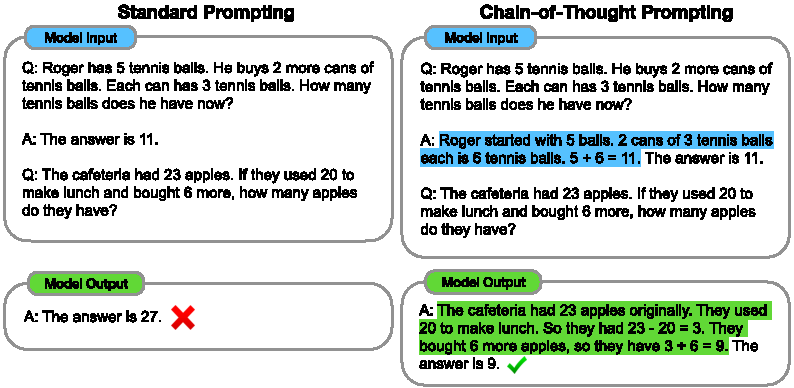
\includegraphics[width=\textwidth]{figures/CoT_picture.pdf}
  \caption{Comparison of standard prompting and
    chain-of-thought prompting. Chain-of-thought
    reasoning steps are highlighted \cite{wei2023}.}
  \label{fig:cot-example}
\end{figure}

\subsection*{Advantages}
Chain-of-thought prompting offers several notable
  advantages. It allows models to
  decompose multi-step problems into intermediate steps,
  allocating more computation to problems that require
  longer reasoning. It also provides an interpretable
  view into the model's reasoning process, making it
  possible to identify where errors occur. Finally, chain-of-thought reasoning
  requires no additional training or fine-tuning ---
  it is elicited simply by including step-by-step
  demonstrations in the few-shot prompt.

\subsection*{Limitations}
However, chain-of-thought prompting also has
  limitations relevant to mathematical reasoning. Although chain of thought emulates
  the thought processes of human reasoners, this does
  not confirm whether the model is actually
  \textit{reasoning}. Furthermore, there is no
  guarantee of correct reasoning paths, meaning the
  model can produce plausible-looking but incorrect
  intermediate steps that nonetheless lead to a wrong
  final answer.
\section{Process Reward Models}
\label{sec:prm}
  While fine-tuning and prompting approaches improve the
  accuracy of language models on mathematical tasks, a
  deeper challenge remains: even when achieving correct
  final answers, models can still produce plausible-looking
  reasoning steps that build upon flawed calculations or
  derivations \cite{qwen2025prm}. Process Reward Models \cite{lightman2024} are
  proposed to address this limitation by identifying and
  mitigating errors in intermediate reasoning steps,
  enabling finer-grained supervision of the reasoning
  process.


Two types of reward models exist for evaluating
  mathematical reasoning. Outcome-supervised reward
  models (ORMs) assess only the final answer from model, predicting
  whether a solution is correct or incorrect as a whole
  . A key weakness of this approach
  is that solutions reaching the correct answer through
  incorrect reasoning are misgraded. Process-supervised
  reward models (PRMs), by contrast, assign a score to
  each individual reasoning step, directly identifying
  the location of any errors.

 In this work,
  Qwen2.5-Math-PRM-7B is employed as the process reward
  model to evaluate the reasoning quality of the
  fine-tuned models, as described in
  Section~\ref{sec:models}.

\chapter{Design and Methodology}
\label{chap:design}
This chapter presents the design of the solution
  developed in this thesis. It begins with an
  analysis of the problem and the goals of the
  work, followed by a description of the GSM8K
  dataset used for training and evaluation. The
  selected language models are then introduced,
  covering their key characteristics and the
  motivation behind their selection. The chapter
  concludes with the fine-tuning strategy,
  describing the training pipeline, evaluation
  methodology, and the hyperparameters adjusted
  throughout the experimental process.
\section{Current Limitations and Research Goals}
\label{sec:problem-analysis}


  Despite the general capabilities of large
  language models described in the preceding
  chapters, mathematical reasoning remains a
  persistent challenge. Even models with billions of
  parameters frequently produce incorrect results on multi-step
  arithmetic problems, making errors in intermediate calculations,
  losing track of previously computed values, or generating answers
  in inconsistent formats \cite{cobbe2021}.

  This makes mathematics a well-established benchmark
  for evaluating and improving the
  problem-solving ability of large language
  models \cite{hendrycks2021}. Unlike many natural language tasks,
  mathematics is grounded in logic and governed by clearly defined
  rules --- each problem has an unambiguous correct answer, and the
  quality of a solution can be assessed objectively. This consistency
  makes experimental results directly comparable across models and
  configurations, and ensures that improvements in benchmark
  performance reflect genuine gains in reasoning ability.

  Although LLMs are pre-trained on large corpora
  from the web \cite{raiaan2024}, this data is
  not primarily focused on structured mathematical
  reasoning, which motivates domain-specific
  fine-tuning as a practical solution.
  Low-Rank Adaptation (LoRA), described in
  Section~\ref{fine-tuning}, was selected as
  the training approach due to its computational
  efficiency \cite{hu2022lora}. Three models
  representing different pre-training approaches
  were selected: Llama-2-7b-hf,
  Llama-2-7b-chat-hf, and
  Mistral-7B-Instruct-v0.1, each described in
  Section~\ref{sec:models}.


  The work pursues the following goals:

  \begin{enumerate}
      \item Fine-tune three LLMs of different pre-training types
      using LoRA on the GSM8K training set.
      \item Conduct a systematic hyperparameter search to identify
      effective LoRA training configurations for each model type.
      \item Evaluate the accuracy of each fine-tuned model on the
      GSM8K test set and compare results against the respective
      pre-fine-tuning baseline.
      \item Assess the quality of mathematical reasoning in
      fine-tuned models using a Process Reward Model as a
      secondary evaluation metric.
  \end{enumerate}


\section{GSM8K Dataset}
\label{sec:gsm8k}



GSM8K (Grade School Math 8K)  \cite{cobbe2021} is a dataset of 8,500 high-quality
  elementary mathematics word problems created by human problem
  writers. The dataset is divided into 7,473
  training problems and 1,319 test problems. Each problem requires
  between two and eight steps to solve, relying exclusively on basic
  arithmetic operations (addition, subtraction, multiplication, and
  division). The problems are designed to be solvable by a bright middle
  school student (approximately 12--14 years of age), yet challenging enough for large
  language models
  to make them a meaningful measure of reasoning ability.

  GSM8K was selected as the training and evaluation dataset for
  this work based on two of its core design properties. First,
  the dataset is constructed with high quality in mind --- rather
  than relying on error-prone scraping procedures, all problems
  were created by human writers and subjected to extensive quality
  control. As a result, the authors estimate that fewer
  than two percent of problems contain breaking
  errors, making the dataset
  a reliable foundation for both fine-tuning
  and evaluation. Second, the
  dataset exhibits high diversity --- each problem is deliberately
  constructed to be unique rather than drawn from a shared
  linguistic template, ensuring that test set performance reflects
  genuine generalization rather than memorization of surface
  patterns.

  Each problem consists of a natural language question paired with a
  step-by-step solution written in natural language, followed by a
  final numerical answer marked with the \texttt{\#\#\#\#} delimiter. This
  chain-of-thought solution format, discussed in Section~\ref{sec:cot}, makes GSM8K
  particularly suitable for
  studying the reasoning process of language models, as each
  intermediate step is explicitly recorded. Intermediate
  calculations are annotated with \texttt{<<...>>} tags indicating
  the arithmetic operation performed and its result.
  Figure~\ref{fig:gsm8k-example} shows a representative example from the dataset.

  \begin{figure}[ht]
  \centering
  \fbox{\begin{minipage}{0.97\textwidth}
  \smallskip
  \textbf{question:} Natalia sold clips to 48 of her friends in
  April, and then she sold half as many clips in May. How many
  clips did Natalia sell altogether in April and May?
  \\[6pt]
  \textbf{answer:} Natalia sold 48/2 =
  \texttt{<<48/2=24>>}24 clips in May.
  Natalia sold 48+24 = \texttt{<<48+24=72>>}72 clips altogether
  in April and May. \texttt{\#\#\#\# 72}
  \smallskip
  \end{minipage}}
  \caption{Example from the GSM8K dataset}
  \label{fig:gsm8k-example}
  \end{figure}

\section{Models}
\label{sec:models}

This section describes the models used in this work. Three models
  are selected for fine-tuning, each representing a different
  pre-training paradigm. The last one is used exclusively for
  evaluating the quality of mathematical reasoning produced by the fine-tuned models.

\subsection*{Llama-2-7b-hf}

  Llama 2 \cite{touvron2023} is a family of pretrained and instruction-tuned large
  language models developed by Meta AI and released in 2023. The base variant,
  Llama-2-7b-hf\footnote{\url{https://huggingface.co/meta-llama/Llama-2-7b-hf}}, is a
  decoder-only transformer with seven billion parameters, pretrained
  on two trillion tokens drawn from a new mix of publicly available
  online sources. The model features a context length of 4,096
  tokens.
  The suffix \textit{-hf} indicates that the model weights have
  been converted to a format compatible with the Hugging Face
  \texttt{transformers}\footnote{\url{https://huggingface.co/docs/transformers}} library.
  As a base model, it is trained
  solely to predict the next token, without instruction tuning or
  alignment with human preferences. That is why Llama-2-7b-hf was selected to
  represent this model type in this work,
  serving as the weakest baseline among the
  three models due to the absence of any
  instruction tuning.
  \subsection*{Llama-2-7b-chat-hf}
  Llama-2-7b-chat-hf\footnote{\url{https://huggingface.co/meta-llama/Llama-2-7b-chat-hf}}
  \cite{touvron2023} is the instruction-tuned counterpart of
  Llama-2-7b-hf, fine-tuned for dialogue applications using
  supervised fine-tuning (SFT) followed by Reinforcement Learning
  with Human Feedback (RLHF), employing rejection sampling and Proximal Policy
  Optimization (PPO). The
  underlying architecture is identical to the base variant: seven
  billion parameters and a context length of 4,096 tokens. Through
  the RLHF process, the model is aligned with human preferences
  and optimized for multi-turn conversational interaction.

This model was selected to represent the chat model type and to enable a direct comparison
  with Llama-2-7b-hf. Since both models share the same base
  architecture and differ only in the post-pretraining alignment
  process, comparing their fine-tuning results isolates the effect
  of RLHF on LoRA adaptation effectiveness.

\subsection*{Mistral-7B-Instruct-v0.1}
Mistral-7B-Instruct-v0.1\footnote{\url{https://huggingface.co/mistralai/Mistral-7B-Instruct-v0.1}}
\cite{jiang2023} is an instruction-tuned version of
  Mistral 7B, a language model with seven billion parameters developed
  by Mistral AI and released in October 2023. The
  instruct variant was obtained by fine-tuning the base model on
  publicly available instruction datasets from the Hugging Face
  repository, without the use of proprietary data or reinforcement
  learning from human feedback.

  Mistral-7B-Instruct-v0.1 was selected to represent the instruct
  model type. Unlike
  Llama-2-7b-chat-hf, which applies RLHF on top of supervised
  fine-tuning, this model relies solely on SFT, making it a
  representative of a distinct alignment approach and completing
  the comparison across all three pre-training paradigms defined
  in this work.


\subsection*{Qwen2.5-Math-PRM-7B}
Qwen2.5-Math-PRM-7B\footnote{\url{https://huggingface.co/Qwen/Qwen2.5-Math-PRM-7B}}
\cite{qwen2025prm} is a Process Reward Model (PRM) developed
  by the Qwen team and used in this work for evaluating the quality
  of mathematical reasoning produced by the fine-tuned models. The model is initialized
  from the supervised
  fine-tuned Qwen2.5-Math-7B-Instruct, where the original language
  modeling head used for next token prediction is replaced with a
  scalar-value head consisting of two linear layers, which assigns
  a score to each individual reasoning step.

  Qwen2.5-Math-PRM-7B was selected due to its strong performance
  in both Best-of-N evaluation and step-wise error identification
  on ProcessBench \cite{zheng-etal-2025-processbench, qwen2025prm}, making it a reliable
  tool
  for assessing whether the reasoning process produced by a model
  is mathematically sound --- independently of whether the final
  answer is correct.
\section{Fine-tuning Strategy}
\label{sec:finetuning-strategy}

To improve mathematical reasoning capabilities, LoRA was adopted as the fine-tuning approach for all three models due to its computational efficiency \cite{hu2022lora}. The work is organized into four stages: baseline evaluation, LoRA fine-tuning, accuracy evaluation, and process reward model scoring.

\subsection{Baseline evaluation}
Before any fine-tuning is applied, each model is evaluated on
  the full GSM8K test set in its original pre-trained state,
  without any LoRA adapter. This baseline serves as a reference
  point for measuring the improvement achieved through fine-tuning.
  To ensure a fair comparison, the baseline evaluation follows the
  same procedure as the post-fine-tuning evaluation: the model
  generates a response for each test example using greedy
  decoding, the numerical answer is extracted from the output, and
  correctness is determined by exact comparison with the ground
  truth. Since base models receive no instruction tuning and
  therefore have no prior understanding of how to follow instructions,
  3-shot examples are prepended to the prompt to guide the
  model toward producing a structured response. In addition, process reward
  model scoring is applied to the baseline outputs to establish a
  reference for reasoning quality prior to fine-tuning, enabling
  a direct comparison of reasoning step quality before and after
  adaptation.

\subsection{LoRA Fine-tuning}
This section describes the key aspects of the
  LoRA fine-tuning process, namely the validation
  strategy, early stopping mechanism, and the
  description of hyperparameters that were
  adjusted across experiments.




\subsection*{Validation split}
To monitor model performance during training, the last 15\% of
  the training examples are reserved as a validation set.
  Rather than
  relying solely on training loss as a progress indicator,
  validation accuracy is measured at regular intervals through
  actual model inference on the validation examples. This
  distinction is important: loss reflects how well the model
  predicts tokens under teacher-forcing, which does not
  necessarily correlate with the model's ability to generate
  correct answers autoregressively. By evaluating real generation
  quality during training, the validation accuracy provides a more
  faithful signal of the model's mathematical reasoning
  performance.

\subsection*{Early stopping}
To prevent overfitting and avoid unnecessary computation, early
  stopping is applied during training. Training is halted when
  validation accuracy fails to improve by more than a minimum
  threshold over six consecutive evaluation steps.

\subsection*{Training Hyperparameters}
The following parameters were adjusted across experiments to
  identify the most effective training configuration:
\begin{itemize}
      \item \textbf{Learning Rate}: Defines how much the model's
      weights are adjusted during each training step.
      \item \textbf{LoRA Rank} ($r$): Controls the number of
      trainable parameters in the LoRA adapter matrices. A higher
      rank increases model capacity but also memory usage.
      \item \textbf{LoRA Alpha} ($\alpha$): Scales the strength
      of the LoRA adjustments in relation to the rank $r$.
      \item \textbf{Epochs}: Number of complete passes through
      the training dataset during fine-tuning.
      \item \textbf{LoRA Dropout}: A regularization technique
      that randomly sets a fraction of LoRA activations to zero
      during training to prevent overfitting.
      \item \textbf{Effective Batch Size}: Total number of
      training examples processed per gradient update, computed
      as the product of batch size and gradient accumulation steps.
  \end{itemize}

\subsection{Accuracy evaluation}
For this work, accuracy was selected as the primary evaluation
  metric, defined as the ratio of correct model answers to the
  total number of examples in the test split (1319 examples). Since
  each GSM8K problem has a single unambiguous numerical solution,
  it provides a straightforward and objective measure of
  mathematical reasoning performance.

\subsection{PRM evaluation}
Process Reward Model evaluation serves as a secondary metric
  that assesses the quality of mathematical reasoning
  independently of the final answer. A model may arrive at a
  correct answer through flawed intermediate steps, or produce
  a well-reasoned solution that nonetheless results in an
  incorrect answer --- accuracy alone cannot distinguish between
  these cases. PRM evaluation addresses this limitation by
  assigning a score to each individual reasoning step produced
  by the model.

  The model output for each example is divided into individual
  reasoning steps, which are then scored by Qwen2.5-Math-PRM-7B.
  Three aggregate scores are computed per example:

  \begin{itemize}
      \item \textbf{Average score}: the mean score across all
      reasoning steps, reflecting the overall quality of the
      reasoning process.
      \item \textbf{Minimum score}: the score of the weakest
      step, capturing the idea that a reasoning chain is only
      as reliable as its least confident step.
     \item \textbf{Product score}: the product of all step
  scores, computed in logarithmic space for
  numerical stability --- specifically as
  $\exp\!\left(\sum \log(s_i + \varepsilon)\right)$,
  where $\varepsilon = 10^{-10}$ prevents
  $\log(0)$. This is mathematically equivalent
  to the direct product but avoids floating-point
  underflow when multiplying many small values.
  Because each score lies in $[0, 1]$, a single
  low-scoring step drives the entire product
  toward zero, making this metric more sensitive
  to individual reasoning errors than the average
  score.
  \end{itemize}
  The per-example scores are aggregated into global
  metrics to enable consistent comparison across
  experiments and models. The following global metrics
  are reported:

  \begin{itemize}
      \item \textbf{Global average step score (avg\_step)}: the
      mean of per-example average scores across all
      evaluated examples.
      \item \textbf{Global average minimum score (avg\_min)}:
      the mean of per-example minimum scores.
      \item \textbf{Global average product score (avg\_prod)}:
      the mean of per-example product scores across
      all examples.
      \item \textbf{Average score correct answers (avg\_correct)}:
      the mean average step score restricted to
      examples where the final answer was correct.
      \item \textbf{Average score incorrect answers (avg\_incorrect)}:
      the mean average step score for examples where
      the final answer was incorrect.
      \item \textbf{Product score correct / incorrect
      answers (prod\_correct, prod\_incorrect)}: analogous product-based scores
      computed separately for correct and incorrect
      examples.
      \item \textbf{High-confidence step rate (high\_conf)}: the
      proportion of individual reasoning steps that
      received a score above 0.8.
  \end{itemize}
  PRM evaluation is applied to both baseline and fine-tuned
  model outputs.
\chapter{Implementation}
\label{chap:implementation}
This chapter describes the implementation of the
  solution designed in Chapter~\ref{chap:design}.
  It covers the dataset preparation pipeline, the
  fine-tuning setup including the key technical
  decisions made during development, and the
  evaluation framework used to assess model
  performance.
\section{Dataset Preparation}
\label{sec:dataset-prep}
The GSM8K dataset is downloaded from the
  Hugging Face Hub using the \texttt{datasets}
  library (version 4.4.1) and converted into
  a JSONL format suitable for fine-tuning.
  Since the three selected models differ in
  their expected input format, a dedicated
  data preparation script applies a
  model-specific formatting step via the
  \texttt{--model-type} argument.

  The \texttt{base} format represents the simplest
  case --- the example is stored as a plain text field
  containing the question and answer separated by a
  newline:

  \begin{lstlisting}
  {"text": "Question: Natalia sold clips...\nAnswer: ..."}
  \end{lstlisting}

  The \texttt{chat} format, used for Llama-2-7b-chat-hf,
  structures the example as a three-turn conversation
  with explicit \texttt{system}, \texttt{user}, and
  \texttt{assistant} roles:

  \begin{lstlisting}
  {"messages": [
    {"role": "system", "content": "You are a helpful..."},
    {"role": "user",   "content": "Natalia sold..."},
    {"role": "assistant", "content": "...#### 72"}
  ]}
  \end{lstlisting}

  The \texttt{instruct} format, used for
  Mistral-7B-Instruct-v0.1, merges the system
  instruction and the question into a single
  \texttt{user} message, as this model does not
  support a separate system role:

  \begin{lstlisting}
  {"messages": [
    {"role": "user",      "content": "You are a helpful...
                                      \n\nNatalia sold..."},
    {"role": "assistant", "content": "...#### 72"}
  ]}
  \end{lstlisting}

  The formatted examples are saved to a JSONL file,
  with one JSON object per line.

\section{Fine-tuning Pipeline}
\label{sec:finetuning-pipeline}
This section describes the key aspects of the
  fine-tuning pipeline implementation, along with
  the versions of libraries used in this work in Table~\ref{tab:libraries}.

  \begin{table}[ht]
  \caption{Libraries used in the fine-tuning
  pipeline.}
  \centering
  \begin{tabular}{ll}
  \toprule
  \textbf{Library} & \textbf{Version} \\
  \midrule
  transformers & 4.57.3 \\
  peft & 0.18.0 \\
  torch & 2.9.1 (CUDA 12.8) \\
  wandb & 0.23.1 \\
  datasets & 4.4.1 \\
  numpy & 2.3.5 \\
  tqdm & 4.67.1 \\
  \bottomrule
  \end{tabular}
  \label{tab:libraries}
  \end{table}

  \subsubsection*{Tokenization and Loss Masking}
    Tokenization for training is handled by two
  functions depending on the model type. In both cases,
  prompt tokens are masked with the value $-100$, which
  is ignored by the cross-entropy loss function, ensuring
  that the model learns to generate only the assistant
  response.

  For \texttt{chat} and \texttt{instruct} models,
  \texttt{tokenize\_chat} function determines the prompt length
  by tokenizing the conversation without the final
  assistant turn, then masks all preceding tokens.

  For \texttt{base} models, \texttt{tokenize\_base} function
  locates the \textit{last} occurrence of
  \texttt{\textbackslash nAnswer:} in the token
  sequence to determine the masking boundary, ensuring
  correct behaviour even if this token sequence appears
  multiple times. All sequences are truncated to a
  maximum length of 512 tokens.

  \subsubsection*{Validation Accuracy Callback}
 A custom callback evaluates the model's actual
  generation performance at regular intervals
  defined by the \texttt{--eval-steps}
  hyperparameter. Rather than monitoring training
  loss, the callback runs batched inference on
  the validation set. During batch generation,
  inputs are left-padded, as required for correct
  autoregressive decoding with variable-length
  sequences.

  For base models, a custom stopping criterion
  is applied, which halts generation as soon as
  the \texttt{\#\#\#\#} answer delimiter appears
  in the output, as base models tend to loop and
  repeat content indefinitely.


\section{Evaluation Framework}
\label{sec:evaluation}
Model evaluation consists of two stages:
  accuracy comparison and PRM scoring.

  The fine-tuned model generates a response
  for each example in the GSM8K test set using
  greedy decoding. The extracted answers are
  then compared against the ground truth from
  the dataset, and the full results --- including
  the question, model output, and correctness
  label --- are saved to a JSON file, which
  serves as input for the PRM evaluation.

  PRM scoring starts from dividing each example
  from model output into individual reasoning steps using a
  hierarchical splitting strategy. The text is first split by
  double newlines (\texttt{\textbackslash n\textbackslash n}),
  and each resulting block is further split by single
  newlines (\texttt{\textbackslash n}). This handles
  both paragraph-style and numbered-step reasoning
  formats.

  The steps are then joined using the special separator
  token \texttt{<extra\_0>}, which Qwen2.5-Math-PRM-7B
  uses to delimit reasoning steps. A single forward
  pass over the entire solution is performed, and the
  PRM score for each step is read from the model's
  output at the positions of the \texttt{<extra\_0>}
  tokens. These step-level scores are then used to compute
  the aggregate evaluation metrics described in
  Section~\ref{sec:finetuning-strategy}.
\chapter{Experiments and Results}
\label{chap:experiments}
This chapter presents the experimental evaluation
  of LoRA fine-tuning applied to the three selected
  models on the GSM8K dataset. All experiments were
  conducted on the MetaCentrum HPC
  cluster\footnote{\url{https://metavo.metacentrum.cz/}}.
  Two metrics were used to evaluate the
  experiments: accuracy on the GSM8K test set as
  the primary metric, and process reward model
  scoring as a secondary metric assessing the
  quality of intermediate reasoning steps. The
  chapter begins with a baseline evaluation of all three models, followed by a description
  of the
  hyperparameter search and its results, then an analysis of reasoning quality using the
  process reward model, and concludes with a
  discussion of the findings.
\section{Baseline Evaluation}
    Prior to the hyperparameter search, each model was
  evaluated on the full GSM8K test set without any
  fine-tuning to establish a baseline. For the base
  model (Llama-2-7b-hf), three-shot examples were
  prepended to each prompt to guide the output format,
  as described in Section~\ref{sec:finetuning-strategy}.
  The baseline results are summarised in
  Table~\ref{tab:baseline}.

  \begin{table}[ht]
  \caption{Baseline accuracy on the GSM8K test set
  before fine-tuning.}
  \centering
  \begin{tabular}{lcc}
  \toprule
  \textbf{Model} & \textbf{Accuracy} & \textbf{Correct / Total} \\
  \midrule
  Llama-2-7b-hf           & 10.77\% & 142 / 1319 \\
  Llama-2-7b-chat-hf      & 25.47\% & 336 / 1319 \\
  Mistral-7B-Instruct-v0.1 & 42.23\% & 557 / 1319 \\
  \bottomrule
  \end{tabular}

  \label{tab:baseline}
  \end{table}

Mistral-7B-Instruct-v0.1 achieves the highest baseline accuracy of
  42.23\%, consistent with the stronger mathematical capabilities of
  the underlying base model --- Mistral 7B  scores 52.2\% on GSM8K
  compared to 16.0\% for Llama-2-7b (8-shot, maj@8)
  \cite{jiang2023}. Llama-2-7b-hf scores only 10.77\%: as a
  raw base model with no instruction tuning, it lacks the ability to
  consistently follow the structured reasoning format and frequently
  produces malformed or incomplete answers. Llama-2-7b-chat-hf reaches
  25.47\%, demonstrating that SFT and RLHF alignment substantially
  improve structured output, yet the result remains constrained by
  the weaker underlying base model.

\section{Hyperparameter Search}
\label{sec:hyperparam-search}
Hyperparameter search is the process of systematically
  evaluating different combinations of training
  parameters to identify configurations that maximise
  model performance. Rather than testing all possible
  combinations simultaneously, this search was structured as four sequential experiments:
  the
  first identified a reference configuration through
  a broad sweep of learning rate and rank values,
  which was then used as the fixed base for three
  independent ablation experiments, each focusing on one aspect of the training
  configuration. This approach allowed
  each hyperparameter to be studied in isolation while
  keeping the overall number of runs manageable.

  Three parameters remained fixed across all four experiments:
  training ran for up to 15 epochs with early stopping (patience~=~6),
  LoRA dropout was set to 0.05, and the random seed was fixed at 42
  to ensure reproducibility.

  \subsection{Experiment 1: Initial Parameter Search}

  The goal of the first experiment was to identify a
  strong reference configuration --- specifically, the
  combination of learning rate and LoRA hyperparameters. The best-performing
  configuration from this experiment was then used as
  the fixed reference point for the subsequent three
  ablation experiments. Each model was evaluated across
  13 configurations combining different learning rates
  and rank values, with $\alpha = 2r$ in all cases.

For Llama-2-7b-hf and Llama-2-7b-chat-hf, learning rates in the
  range 5e-5 to 1e-3 were explored across ranks
  $r \in \{16, 32, 64\}$. Both models achieved their best results at
  lr=3e-4, r=32: 32.98\% for Llama-2-7b-hf (+22.2\% over
  baseline) and 38.51\% for Llama-2-7b-chat-hf (+13.0\%). For
  Llama-2-7b-chat-hf, very low learning rates (2e-5,
  5e-5) produced negligible improvement of only +0.2--0.5\%,
  indicating that the  model requires a sufficiently large
  update step to acquire new mathematical knowledge. Additionally, rank $r=64$ yielded
  noticeably lower accuracy than
  $r=32$ for Llama-2-7b-hf (30.17\% vs.\ 32.98\%), while for
  Llama-2-7b-chat-hf the difference was negligible (38.21\%
  vs.\ 38.51\%). The results are shown in Tables~\ref{tab:exp1-llama-hf}
  and~\ref{tab:exp1-llama-chat}.
\begin{table}[ht]
  \caption{Experiment 1 results --- Llama-2-7b-hf (baseline: 10.77\%). Reference configuration search over learning rate and LoRA rank.}
  \centering
  \footnotesize
  \begin{tabular}{lcccrr}
  \toprule
  \textbf{lr} & \textbf{r} & \textbf{$\alpha$} & \textbf{Accuracy} & \textbf{$\Delta$ baseline} \\
  \midrule
  5e-5 & 16 & 32 & 24.18\% & +13.4\% \\
  1e-4 & 16 & 32 & 27.45\% & +16.7\% \\
  2e-4 & 16 & 32 & 28.66\% & +17.9\% \\
  8e-4 & 16 & 32 & 31.01\% & +20.2\% \\
  1e-3 & 16 & 32 & 28.13\% & +17.4\% \\
  \midrule
  \textbf{3e-4} & \textbf{32} & \textbf{64} & \textbf{32.98\%} & \textbf{+22.2\%} \\
  5e-4 & 32 & 64 & 30.25\% & +19.5\% \\
  6e-4 & 32 & 64 & 28.96\% & +18.2\% \\
  8e-4 & 32 & 64 & 27.60\% & +16.8\% \\
  1e-3 & 32 & 64 & 26.46\% & +15.7\%\\
  \midrule
  2e-4 & 64 & 128 & 30.17\% & +19.4\% \\
  5e-4 & 64 & 128 & 26.76\% & +16.0\% \\
  8e-4 & 64 & 128 & 26.54\% & +15.8\% \\
  \bottomrule
  \end{tabular}

  \label{tab:exp1-llama-hf}
  \end{table}
  \hfill
  \begin{table}[ht]
  \caption{Experiment 1 results --- Llama-2-7b-chat-hf (baseline: 25.47\%). Reference configuration search over learning rate and LoRA rank.}
  \centering
  \footnotesize
  \begin{tabular}{lcccrr}
  \toprule
  \textbf{lr} & \textbf{r} & \textbf{$\alpha$} & \textbf{Accuracy} & \textbf{$\Delta$ baseline} \\
  \midrule
  2e-5 & 16 & 32 & 25.93\% & +0.5\% \\
  5e-5 & 16 & 32 & 25.70\% & +0.2\% \\
  1e-4 & 16 & 32 & 35.78\% & +10.3\%\\
  8e-4 & 16 & 32 & 37.23\% & +11.8\% \\
  1e-3 & 16 & 32 & 34.95\% & +9.5\% \\
  \midrule
  \textbf{3e-4} & \textbf{32} & \textbf{64} & \textbf{38.51\%} & \textbf{+13.0\%} \\
  5e-4 & 32 & 64 & 36.47\% & +11.0\% \\
  6e-4 & 32 & 64 & 38.21\% & +12.7\% \\
  8e-4 & 32 & 64 & 35.48\% & +10.0\% \\
  1e-3 & 32 & 64 & 35.56\% & +10.1\% \\
  \midrule
  2e-4 & 64 & 128 & 36.01\% & +10.5\% \\
  5e-4 & 64 & 128 & 34.50\% & +9.0\% \\
  8e-4 & 64 & 128 & 38.21\% & +12.7\% \\
  \bottomrule
  \end{tabular}

  \label{tab:exp1-llama-chat}
  \end{table}

For Mistral-7B-Instruct-v0.1, a more conservative range of
  5e-6 to 8e-4 was explored. The lowest learning
  rate (5e-6) degraded performance below the baseline
  (41.32\%, $-$0.9\%), while the best configuration
  lr=1e-4, r=64 reached 53.60\% (+11.4\%). Unlike the Llama
  models, the larger rank $r=64$ proved beneficial, and increasing
  the learning rate beyond 1e-4 consistently reduced accuracy,
  reflecting the sensitivity of instruction-tuned models to large
  parameter updates. The results are shown in Tables~\ref{tab:exp1-mistral}.

  \begin{table}[ht]
  \caption{Experiment 1 results --- Mistral-7B-Instruct-v0.1 (baseline: 42.23\%). Reference configuration search over learning rate and LoRA rank.}
  \centering
  \footnotesize
  \begin{tabular}{lcccrr}
  \toprule
  \textbf{lr} & \textbf{r} & \textbf{$\alpha$} & \textbf{Accuracy} & \textbf{$\Delta$ baseline} \\
  \midrule
    5e-6   & 16 & 32 & 41.32\% & -0.9\% \\
    1.5e-5 & 16 & 32 & 53.15\% & +10.9\%\\
    5e-5   & 16 & 32 & 52.77\% & +10.5\% \\
  \midrule
  2e-4 & 32 & 64 & 51.78\% & +9.6\% \\
  3e-4 & 32 & 64 & 52.39\% & +10.2\% \\
  5e-4 & 32 & 64 & 51.18\% & +9.0\% \\
  6e-4 & 32 & 64 & 48.98\% & +6.8\% \\
  8e-4 & 32 & 64 & 51.18\% & +9.0\% \\
  \midrule
  \textbf{1e-4} & \textbf{64} & \textbf{128} & \textbf{53.60\%} & \textbf{+11.4\%} \\
  2e-4 & 64 & 128 & 48.82\% & +6.6\% \\
  3e-4 & 64 & 128 & 50.57\% & +8.3\% \\
  5e-4 & 64 & 128 & 51.78\% & +9.6\% \\
  8e-4 & 64 & 128 & 46.47\% & +4.2\% \\
  \bottomrule
  \end{tabular}

  \label{tab:exp1-mistral}
  \end{table}
The selected reference configurations are lr=3e-4, r=32
  for both Llama models, and lr=1e-4, r=64 for
  Mistral-7B-Instruct-v0.1. The contrast between the two groups is
  notable: both Llama models require higher learning rates and smaller
  rank, whereas Mistral converges at a lower learning rate with a
  larger rank --- consistent with the expectation that instruction-tuned
  models are more sensitive to aggressive parameter updates.

\subsection{Experiment 2: Effective Batch Size}

  The goal of this experiment was to determine the
  optimal effective batch size, defined as the product
  of the physical batch size and the number of gradient
  accumulation steps. Since the physical batch size was
  fixed at 4, and only the
  gradient accumulation steps were varied. All other
  parameters were set to the best configuration
  identified in Experiment 1.

For both Llama models (Tables~\ref{tab:exp2-llama-hf}
  and~\ref{tab:exp2-llama-chat}), eff\_batch=128 is
  confirmed as optimal, with accuracy dropping at both
  smaller and larger effective batch values.

  \begin{table}[ht]
  \caption{Experiment 2 results (effective batch size ablation) --- Llama-2-7b-hf (baseline: 10.77\%).}
  \centering
  \footnotesize
  \begin{tabular}{lccrr}
  \toprule
  \textbf{eff\_batch} & \textbf{Accuracy} & \textbf{$\Delta$ baseline} & \textbf{$\Delta$ ref} \\
  \midrule
  32  & 28.51\% & +17.7\% & -4.47\% \\
  64  & 30.86\% & +20.1\% & -2.12\% \\
  \textbf{128 (ref)} & \textbf{32.98\%} & \textbf{+22.2\%} & \textbf{---} \\
  256 & 29.64\% & +18.9\% & -3.34\% \\
  512 & 29.11\% & +18.3\% & -3.87\% \\
  \bottomrule
  \end{tabular}

  \label{tab:exp2-llama-hf}
  \end{table}

  \begin{table}[ht]
  \caption{Experiment 2 results (effective batch size ablation) --- Llama-2-7b-chat-hf (baseline: 25.47\%).}
  \centering
  \footnotesize
  \begin{tabular}{lccrr}
  \toprule
  \textbf{eff\_batch} & \textbf{Accuracy} & \textbf{$\Delta$ baseline} & \textbf{$\Delta$ ref} \\
  \midrule
  32  & 36.01\% & +10.5\% & -2.50\% \\
  64  & 37.23\% & +11.8\% & -1.28\% \\
  \textbf{128 (ref)} & \textbf{38.51\%} & \textbf{+13.0\%} & \textbf{---} \\
  256 & 35.86\% & +10.4\% & -2.65\% \\
  512 & 34.72\% & +9.3\%  & -3.79\% \\
  \bottomrule
  \end{tabular}

  \label{tab:exp2-llama-chat}
  \end{table}
  Mistral-7B-Instruct-v0.1 (Table~\ref{tab:exp2-mistral}) shows a
  different pattern: eff\_batch=64 achieves the best accuracy
  at 55.95\%, surpassing the reference (eff\_batch=128,
  53.60\%) by 2.35\%. This indicates that Mistral benefits from more
  frequent gradient updates, likely due to its lower learning rate
  requiring more parameter update steps to converge.

  \begin{table}[ht]
  \caption{Experiment 2 results (effective batch size ablation) --- Mistral-7B-Instruct-v0.1 (baseline: 42.23\%).}
  \centering
  \footnotesize
  \begin{tabular}{lccrr}
  \toprule
  \textbf{eff\_batch} & \textbf{Accuracy} & \textbf{$\Delta$ baseline} & \textbf{$\Delta$ ref} \\
  \midrule
  32  & 51.48\% & +9.3\%  & -2.12\% \\
  \textbf{64}  & \textbf{55.95\%} & \textbf{+13.7\%} & \textbf{+2.35\%} \\
  128 (ref) & 53.60\% & +11.4\% & --- \\
  256 & 54.06\% & +11.8\% & +0.46\% \\
  512 & 50.42\% & +8.2\%  & -3.18\% \\
  \bottomrule
  \end{tabular}

  \label{tab:exp2-mistral}
  \end{table}

  In summary, the optimal effective batch size is
  128 for both Llama models and 64 for
  Mistral.


\subsection{Experiment 3: Learning Rate Ablation}

  The goal of this experiment was to refine the learning rate search
  by evaluating finer-grained values in the neighbourhood of the
  optimum identified in Experiment~1. All other parameters
  were fixed at the Experiment 1 reference configuration.

  \begin{table}[ht]
  \caption{Experiment 3 results (fine-grained learning rate search) --- Llama-2-7b-hf (baseline: 10.77\%).}
  \centering
  \footnotesize
  \begin{tabular}{lcccrr}
  \toprule
  \textbf{LR} & \textbf{Source} & \textbf{Accuracy} & \textbf{$\Delta$ baseline} & \textbf{$\Delta$ ref} \\
  \midrule
  5e-5  & Exp 3 & 27.22\% & +16.4\% & -5.76\% \\
  1e-4  & Exp 3 & 27.75\% & +17.0\% & -5.23\% \\
  1.5e-4 & Exp 3 & 30.93\% & +20.2\% & -2.05\% \\
  2e-4  & Exp 3 & 31.31\% & +20.5\% & -1.67\% \\
  2.5e-4 & Exp 3 & 30.93\% & +20.2\% & -2.05\% \\
  \textbf{3e-4 (ref)} & \textbf{Exp 1} & \textbf{32.98\%} & \textbf{+22.2\%} & \textbf{---} \\
  3.5e-4 & Exp 3 & 30.78\% & +20.0\% & -2.20\% \\
  4e-4  & Exp 3 & 29.42\% & +18.7\% & -3.56\% \\
  4.5e-4 & Exp 3 & 29.26\% & +18.5\% & -3.72\% \\
  5e-4  & Exp 1 & 30.25\% & +19.5\% & -2.73\% \\
  6e-4  & Exp 1 & 28.96\% & +18.2\% & -4.02\% \\
  8e-4  & Exp 1 & 27.60\% & +16.8\% & -5.38\% \\
  1e-3  & Exp 1 & 26.46\% & +15.7\% & -6.52\% \\
  \bottomrule
  \end{tabular}

  \label{tab:exp3-llama-hf}
  \end{table}

  Llama-2-7b-hf (Table~\ref{tab:exp3-llama-hf}) confirms
  lr=3e-4 as the optimal learning rate (32.98\%). Values below the optimum rise
  gradually --- from 27.22\% at 5e-5 to 31.31\% at
  2e-4 --- while values above decline steadily, reaching
  26.46\% at 1e-3.

  \begin{table}[ht]
  \caption{Experiment 3 results (fine-grained learning rate search) --- Llama-2-7b-chat-hf (baseline: 25.47\%).}
  \centering
  \footnotesize
  \begin{tabular}{lcccrr}
  \toprule
  \textbf{LR} & \textbf{Source} & \textbf{Accuracy} & \textbf{$\Delta$ baseline} & \textbf{$\Delta$ ref} \\
  \midrule
  5e-5   & Exp 3 & 34.57\% & +9.1\%  & -3.94\% \\
  1e-4   & Exp 3 & 38.67\% & +13.2\% & +0.16\% \\
  \textbf{1.5e-4} & \textbf{Exp 3} & \textbf{39.88\%} & \textbf{+14.4\%} & \textbf{+1.37\%} \\
  2e-4   & Exp 3 & 33.21\% & +7.7\%  & -5.30\% \\
  2.5e-4 & Exp 3 & 36.69\% & +11.2\% & -1.82\% \\
  3e-4 (ref) & Exp 1 & 38.51\% & +13.0\% & --- \\
  3.5e-4 & Exp 3 & 37.38\% & +11.9\% & -1.13\% \\
  4e-4   & Exp 3 & 35.56\% & +10.1\% & -2.95\% \\
  4.5e-4 & Exp 3 & 36.54\% & +11.1\% & -1.97\% \\
  5e-4   & Exp 1 & 36.47\% & +11.0\% & -2.04\% \\
  6e-4   & Exp 1 & 38.21\% & +12.7\% & -0.30\% \\
  8e-4   & Exp 1 & 35.48\% & +10.0\% & -3.03\% \\
  1e-3   & Exp 1 & 35.56\% & +10.1\% & -2.95\% \\
  \bottomrule
  \end{tabular}

  \label{tab:exp3-llama-chat}
  \end{table}

  For Llama-2-7b-chat-hf (Table~\ref{tab:exp3-llama-chat}),
  lr=1.5e-4 achieves the best accuracy at 39.88\%,
  surpassing the Experiment 1 reference by 1.37\%.
  The result for lr=2e-4 (33.21\%) is noticeably
  lower than for neighbouring values --- 39.88\%
  for lr=1.5e-4 and 36.69\% for lr=2.5e-4 ---
  indicating a drop of over 6\% that does not
  correspond to the expected smooth trend of the
  learning rate curve. This phenomenon can be
  interpreted as a convergence anomaly.

  \begin{table}[ht]
  \caption{Experiment 3 results (fine-grained learning rate search) --- Mistral-7B-Instruct-v0.1 (baseline: 42.23\%).}
  \centering
  \footnotesize
  \begin{tabular}{lcccrr}
  \toprule
  \textbf{LR} & \textbf{Source} & \textbf{Accuracy} & \textbf{$\Delta$ baseline} & \textbf{$\Delta$ ref} \\
  \midrule
  1e-5   & Exp 3 & 53.60\% & +11.4\% & 0.00\% \\
  2e-5   & Exp 3 & 54.06\% & +11.8\% & +0.46\% \\
  3e-5   & Exp 3 & 52.62\% & +10.4\% & -0.98\% \\
  4e-5   & Exp 3 & 56.41\% & +14.2\% & +2.81\% \\
  5e-5   & Exp 3 & 56.63\% & +14.4\% & +3.03\% \\
  \textbf{6e-5} & \textbf{Exp 3} & \textbf{57.01\%} & \textbf{+14.8\%} & \textbf{+3.41\%} \\
  8e-5   & Exp 3 & 53.98\% & +11.8\% & +0.38\% \\
  1e-4 (ref) & Exp 1 & 53.60\% & +11.4\% & --- \\
  1.5e-4 & Exp 3 & 53.37\% & +11.1\% & -0.23\% \\
  2e-4   & Exp 1 & 48.82\% & +6.6\%  & -4.78\% \\
  3e-4   & Exp 1 & 50.57\% & +8.3\%  & -3.03\% \\
  5e-4   & Exp 1 & 51.78\% & +9.6\%  & -1.82\% \\
  8e-4   & Exp 1 & 46.47\% & +4.2\%  & -7.13\% \\
  \bottomrule
  \end{tabular}

  \label{tab:exp3-mistral}
  \end{table}

  For Mistral-7B-Instruct-v0.1
  (Table~\ref{tab:exp3-mistral}), exploring lower
  learning rates revealed that the true optimum lies
  at lr=6e-5 (57.01\%), which was not covered in
  Experiment 1. This represents a 3.41\% improvement
  over the previous best.

In summary, the learning rate of lr=3e-4 is
  confirmed as optimal for Llama-2-7b-hf. For
  Llama-2-7b-chat-hf, a finer search revealed
  lr=1.5e-4 as the new best configuration. For
  Mistral-7B-Instruct-v0.1, exploring lower values
  showed that the true optimum lies at lr=6e-5.

\subsection{Experiment 4: LoRA Rank and Alpha Ablation}

  This experiment tested two aspects of the LoRA
  configuration independently: rank ablation, where
  the rank was varied with alpha fixed at $\alpha = 2r$,
  and alpha ablation, where the rank was fixed at the
  reference value while alpha was varied. All other
  parameters were set to the Experiment 1 reference
  configuration.

\begin{table}[ht]
\caption{Experiment 4 results (LoRA rank and alpha ablation) --- Llama-2-7b-hf (baseline: 10.77\%).}
  \centering
  \footnotesize
  \begin{tabular}{cccrrr}
  \toprule
  \textbf{r} & \textbf{alpha} & \textbf{alpha/r} & \textbf{Accuracy} & \textbf{$\Delta$ baseline} & \textbf{$\Delta$ ref} \\
  \midrule
  \textbf{32} & \textbf{128} & \textbf{4.0} & \textbf{33.36\%} & \textbf{+22.59\%} & \textbf{+0.38\%} \\
  32  & 64  & 2.0 & 32.98\% & +22.21\% & --- (ref) \\
  64  & 128 & 2.0 & 32.68\% & +21.91\% & -0.30\% \\
  128 & 256 & 2.0 & 31.92\% & +21.15\% & -1.06\% \\
  32  & 32  & 1.0 & 31.46\% & +20.69\% & -1.52\% \\
  16  & 32  & 2.0 & 29.57\% & +18.80\% & -3.41\% \\
  32  & 16  & 0.5 & 29.57\% & +18.80\% & -3.41\% \\
  8   & 16  & 2.0 & 28.35\% & +17.58\% & -4.63\% \\
  4   & 8   & 2.0 & 26.69\% & +15.92\% & -6.29\% \\
  \bottomrule
  \end{tabular}

  \label{tab:exp4-llama-hf}
  \end{table}

  Llama-2-7b-hf (Table~\ref{tab:exp4-llama-hf}) confirms r=32 as
  optimal. Increasing alpha to 128 yields a marginal improvement of
  0.38\% (33.36\%), while larger ranks bring no benefit --- r=64 gives
  32.68\% and r=128 drops to 31.92\%. Very small ranks reduce accuracy
  significantly, falling to 26.69\% at r=4.

\begin{table}[ht]
  \caption{Experiment 4 results (LoRA rank and alpha ablation) --- Llama-2-7b-chat-hf (baseline: 25.47\%).}
  \centering
  \footnotesize
  \begin{tabular}{cccrrr}
  \toprule
  \textbf{r} & \textbf{alpha} & \textbf{alpha/r} & \textbf{Accuracy} & \textbf{$\Delta$ baseline} & \textbf{$\Delta$ ref} \\
  \midrule
  32  & 64  & 2.0 & 38.51\% & +13.04\% & --- (ref) \\
  64  & 128 & 2.0 & 37.23\% & +11.76\% & -1.28\% \\
  32  & 16  & 0.5 & 37.00\% & +11.53\% & -1.51\% \\
  128 & 256 & 2.0 & 36.85\% & +11.38\% & -1.66\% \\
  32  & 32  & 1.0 & 35.78\% & +10.31\% & -2.73\% \\
  8   & 16  & 2.0 & 35.63\% & +10.16\% & -2.88\% \\
  4   & 8   & 2.0 & 35.41\% & +9.94\%  & -3.10\% \\
  32  & 128 & 4.0 & 34.95\% & +9.48\%  & -3.56\% \\
  16  & 32  & 2.0 & 34.72\% & +9.25\%  & -3.79\% \\
  \bottomrule
  \end{tabular}

  \label{tab:exp4-llama-chat}
  \end{table}

  For Llama-2-7b-chat-hf
  (Table~\ref{tab:exp4-llama-chat}), no configuration
  improves upon the reference. Notably, higher alpha
  hurts performance for this model --- r32\_a128 gives
  only 34.95\%, the worst result --- which is the
  opposite of the pattern observed in Llama-2-7b-hf.

 \begin{table}[ht]
  \caption{Experiment 4 result (LoRA rank and alpha ablation) --- Mistral-7B-Instruct-v0.1 (baseline: 42.23\%).}
  \centering
  \footnotesize
  \begin{tabular}{cccrrr}
  \toprule
  \textbf{r} & \textbf{alpha} & \textbf{alpha/r} & \textbf{Accuracy} & \textbf{$\Delta$ baseline} & \textbf{$\Delta$ ref} \\
  \midrule
  \textbf{64} & \textbf{64}  & \textbf{1.0} & \textbf{56.10\%} & \textbf{+13.87\%} & \textbf{+2.50\%} \\
  32  & 64  & 2.0 & 55.95\% & +13.72\% & +2.35\% \\
  16  & 32  & 2.0 & 55.12\% & +12.89\% & +1.52\% \\
  64  & 32  & 0.5 & 55.04\% & +12.81\% & +1.44\% \\
  128 & 256 & 2.0 & 54.44\% & +12.21\% & +0.84\% \\
  64  & 128 & 2.0 & 53.60\% & +11.37\% & --- (ref) \\
  64  & 256 & 4.0 & 53.15\% & +10.92\% & -0.45\% \\
  8   & 16  & 2.0 & 52.84\% & +10.61\% & -0.76\% \\
  4   & 8   & 2.0 & 50.64\% & +8.41\%  & -2.96\% \\
  \bottomrule
  \end{tabular}

  \label{tab:exp4-mistral}
  \end{table}

  Mistral-7B-Instruct-v0.1 (Table~\ref{tab:exp4-mistral}) is the
  only model where multiple configurations outperform the reference.
  The best result is r=64, alpha=64 (56.10\%, +2.50\%), achieved by
  halving the alpha/r ratio from 2.0 to 1.0. This confirms Mistral's
  preference for conservative adapter updates observed throughout
  the experiments.

  Based on the results, the best configuration for
  Llama-2-7b-hf is r=32 with alpha=128 (33.36\%).
  For Llama-2-7b-chat-hf, no configuration improves
  upon the Experiment 1 reference. For
  Mistral-7B-Instruct-v0.1, the results confirm a
  preference for more conservative adapter updates ---
  the best configuration is r=64 with alpha=64.
\section{Process Reward Model Analysis}
\label{sec:prm-analysis}
  Section~\ref{sec:hyperparam-search} evaluated
  model performance exclusively through accuracy,
  without examining the quality of the intermediate
  reasoning steps produced by each model. This
  section extends that analysis by assessing
  reasoning quality using the process reward model.
  PRM scores are compared between the baseline and
  the best fine-tuned configuration for each model:
  Experiment 4 (r=32, $\alpha$=128,
  33.36\%) for Llama-2-7b-hf, Experiment 3
  (lr=1.5e-4, 39.88\%) for Llama-2-7b-chat-hf,
  and Experiment 3 (lr=6e-5, 57.01\%) for
  Mistral-7B-Instruct-v0.1.                                                             
  For each model, a representative example is shown
  with the PRM score assigned to each reasoning step
  indicated in square brackets.

  \subsection{Llama-2-7b-hf}
\begin{table}[ht]
  \caption{PRM step scores --- Llama-2-7b-hf.}
  \centering
  \footnotesize
  \begin{tabular}{lccccc}
  \toprule
  \textbf{Config} & \textbf{avg\_step} & \textbf{avg\_min} & \textbf{avg\_correct} & \textbf{avg\_incorrect} & \textbf{steps} \\
  \midrule
  Baseline           & 0.1130 & 0.1043 & 0.6310 & 0.0505 & 1417 \\
  r=32, $\alpha$=128 & 0.5655 & 0.3005 & 0.8960 & 0.4000 & 6392 \\
  \bottomrule
  \end{tabular}

  \label{tab:prm-llama-hf-1}
  \end{table}

  \begin{table}[ht]
  \caption{PRM product scores --- Llama-2-7b-hf.}
  \centering
  \footnotesize
  \begin{tabular}{lcccc}
  \toprule
  \textbf{Config} & \textbf{avg\_prod} & \textbf{prod\_correct} & \textbf{prod\_incorrect} & \textbf{high\_conf} \\
  \midrule
  Baseline           & 0.1038 & 0.6310 & 0.0402 & 0.0932 \\
  r=32, $\alpha$=128 & 0.2693 & 0.7495 & 0.0289 & 0.4373 \\
  \bottomrule
  \end{tabular}

  \label{tab:prm-llama-hf-2}
  \end{table}
As a base model without any instruction tuning,
  Llama-2-7b-hf is expected to struggle not only
  with mathematical reasoning but also with producing
  structured responses in the first place. The PRM
  results confirm this: the baseline generates only
  1417 reasoning steps across all 1319 examples ---
  roughly one step per example --- because without
  fine-tuning the model produces minimal,
  unstructured outputs that offer little for the
  PRM to evaluate.

  After fine-tuning, the picture changes
  significantly. The number of steps rises to 6392,
  reflecting that the model has learned to produce
  proper chain-of-thought reasoning. Several metrics confirm this improvement:
  avg\_step rises from 0.1130 to 0.5655, avg\_min
  from 0.1043 to 0.3005, and avg\_prod from 0.1038
  to 0.2693, all reflecting higher overall
  reasoning quality. The high\_conf rate increases
  from 0.0932 to 0.4373, indicating that the model
  now regularly produces steps that PRM rates with
  high confidence. Full
  results are presented in
  Tables~\ref{tab:prm-llama-hf-1}
  and~\ref{tab:prm-llama-hf-2}.

The following example illustrates the difference
  in reasoning structure between the baseline and
  fine-tuned versions of the model.                                                       
  \begin{quote}
  \textbf{Question:} A robe takes 2 bolts of blue
  fiber and half that much white fiber. How many
  bolts in total does it take?
  \end{quote}

  \begin{quote}
  \textbf{Baseline:}\\
  \texttt{The robe takes 2 + (1/2) = 3 bolts of
  blue fiber and 3/2 = 1.5 bolts of white fiber. \#\#\#\# 4.5 [0.0117]}
  \end{quote}

  \begin{quote}
  \textbf{Fine-tuned:}\\
  \texttt{The robe takes 2*2=<<2*2=4>>4 bolts of
  blue fiber.\textbackslash n [0.0056]\\
  It takes 2/2=<<2/2=1>>1 bolt of white fiber.\textbackslash n [0.1650]\\
  In total, it takes 4+1=<<4+1=5>>5 bolts.\textbackslash n [0.6680]\\                     
  \#\#\#\# 5 [0.9648]}
  \end{quote}
  The
  baseline produces a single unstructured step that
  receives a PRM score of 0.0117, indicating that
  the reasoning is immediately identified as
  unreliable. The fine-tuned model generates four
  structured steps, however the first step
  --- \texttt{2*2=4 bolts of blue fiber} --- contains
  a conceptual error and receives a score of 0.0056,
  which drives the product score to nearly zero. Both answers are incorrect, yet the
  fine-tuned model's structured format allows PRM
  to precisely locate where the reasoning goes
  wrong --- something impossible with the single-line
  baseline output.

  \subsection{Llama-2-7b-chat-hf}

    \begin{table}[ht]
  \caption{PRM step scores --- Llama-2-7b-chat-hf.}
  \centering
  \footnotesize
  \begin{tabular}{lccccc}
  \toprule
  \textbf{Config} & \textbf{avg\_step} & \textbf{avg\_min} & \textbf{avg\_correct} & \textbf{avg\_incorrect} & \textbf{steps} \\
  \midrule
  Baseline        & 0.7580 & 0.2841 & 0.9483 & 0.6930 & 14040 \\
  lr=1.5e-4 & 0.6252 & 0.3530 & 0.8994 & 0.4434 & 6095 \\
  \bottomrule
  \end{tabular}

  \label{tab:prm-llama-chat-1}
  \end{table}

  \begin{table}[ht]
  \caption{PRM product scores --- Llama-2-7b-chat-hf.}
  \centering
  \footnotesize
  \begin{tabular}{lcccc}
  \toprule
  \textbf{Config} & \textbf{avg\_prod} & \textbf{prod\_correct} & \textbf{prod\_incorrect} & \textbf{high\_conf} \\
  \midrule
  Baseline        & 0.2388 & 0.7454 & 0.0656 & 0.6831 \\
  lr=1.5e-4 & 0.3217 & 0.7489 & 0.0384 & 0.5176 \\
  \bottomrule
  \end{tabular}

  \label{tab:prm-llama-chat-2}
  \end{table}
  Unlike the base model, Llama-2-7b-chat-hf already
  produces structured, multi-step reasoning before
  fine-tuning --- however, the PRM results reveal a
  significant weakness. The baseline generates 14040 steps across the
  test set, with a high\_conf rate of 0.6831,
  reflecting that the majority of these verbose
  steps receive high PRM scores. This inflates
  scores even for incorrect answers --- avg\_incorrect
  reaches 0.6930, nearly as high as avg\_correct
  at 0.9483. This poor discrimination indicates
  that incorrect answers contain reasoning steps
  that appear plausible to the PRM, making it
  difficult to distinguish good from flawed
  reasoning.

  After fine-tuning, avg\_incorrect drops to 0.4434
  and prod\_incorrect decreases from 0.0656 to
  0.0384, reflecting a substantial improvement in
  discrimination. The number of steps also decreases
  to 6095, indicating more concise and focused
  responses. Full
  results are presented in
  Tables~\ref{tab:prm-llama-chat-1}
  and~\ref{tab:prm-llama-chat-2}.

Using the same example question, the contrast
  between the two versions is clear:
\begin{quote}
  \textbf{Baseline:}\\
  \texttt{Great, I'd be happy to help you solve
  this problem! Here's the \\step-by-step solution:\textbackslash n\textbackslash n
  [0.9648]\\
  1. The robe takes 2 bolts of blue fiber.\textbackslash n [1.0000]\\
  2. The robe takes half as much white fiber as
  it takes blue \\fiber.\textbackslash n [0.9727]\\
  3. So, the robe takes 2 x 0.5 = 1 bolt of white
  fiber.\textbackslash n [0.9727]\\
  4. Therefore, the total is 2 + 1 = 3 bolts.\textbackslash n\textbackslash n [0.9883]\\
  So, the final answer is 3 bolts. [0.9961]}
  \end{quote}

  \begin{quote}
  \textbf{Fine-tuned:}\\
  \texttt{The robe takes 2*2=<<2*2=4>>4 bolts of
  blue fiber.\textbackslash n [0.0057]\\
  It takes 2/2=<<2/2=1>>1 bolt of white fiber.\textbackslash n [0.1689]\\
  It takes 4+1=<<4+1=5>>5 bolts in total.\textbackslash n [0.7500]\\
  \#\#\#\# 5  [0.9766]}
  \end{quote}
In this case, the baseline produces the correct
  answer with consistently high PRM scores across
  all steps, confirming well-structured reasoning.
  The fine-tuned model, on the other hand, makes
  an error in the first step which propagates to
  an incorrect final answer. Notably, fine-tuning
  also changed the model's response style --- instead
  of verbose numbered steps, the model now produces
  compact calculations in the GSM8K format.


  \subsection{Mistral-7B-Instruct-v0.1}

  \begin{table}[ht]
  \caption{PRM step scores --- Mistral-7B-Instruct-v0.1.}
  \centering
  \footnotesize
  \begin{tabular}{lccccc}
  \toprule
  \textbf{Config} & \textbf{avg\_step} & \textbf{avg\_min} & \textbf{avg\_correct} & \textbf{avg\_incorrect} & \textbf{steps} \\
  \midrule
  Baseline      & 0.8214 & 0.4694 & 0.9638 & 0.7174 & 12422 \\
  lr=6e-5 & 0.7680 & 0.5353 & 0.9478 & 0.5296 & 6087 \\
  \bottomrule
  \end{tabular}

  \label{tab:prm-mistral-1}
  \end{table}

  \begin{table}[ht]
  \caption{PRM product scores --- Mistral-7B-Instruct-v0.1.}
  \centering
  \footnotesize
  \begin{tabular}{lcccc}
  \toprule
  \textbf{Config} & \textbf{avg\_prod} & \textbf{prod\_correct} & \textbf{prod\_incorrect} & \textbf{high\_conf} \\
  \midrule
  Baseline      & 0.4330 & 0.8363 & 0.1383 & 0.7697 \\
  lr=6e-5 & 0.5035 & 0.8299 & 0.0704 & 0.6905 \\
  \bottomrule
  \end{tabular}

  \label{tab:prm-mistral-2}
  \end{table}
Mistral starts from the strongest baseline
  reasoning quality among the three models,
  reflected in the highest avg\_step (0.8214),
  avg\_correct (0.9638), and prod\_correct (0.8363).  However, the baseline
  avg\_incorrect of 0.7174 and prod\_incorrect of
  0.1383 reveal that incorrect answers still
  receive relatively high scores, indicating
  limited discrimination between correct and
  flawed reasoning.

  After fine-tuning, avg\_incorrect drops from
  0.7174 to 0.5296 and prod\_incorrect decreases
  from 0.1383 to 0.0704 --- nearly halved ---
  indicating substantially improved discrimination.
  The avg\_prod score increases from 0.4330 to
  0.5035, reflecting higher overall reasoning
  quality. The number of steps also decreases from
  12422 to 6087, suggesting more compact and
  precise responses after fine-tuning. Full results are presented in
  Tables~\ref{tab:prm-mistral-1}
  and~\ref{tab:prm-mistral-2}.

  Using the same example question, the following
  outputs illustrate how PRM evaluates the
  reasoning of both versions:
  \begin{quote}
  \textbf{Baseline:}\\
  \texttt{To solve this problem, we need to add
  the amount of blue fiber and white fiber required
  for the robe.\textbackslash n\textbackslash n [0.9961]\\
  1. The robe takes 2 bolts of blue
  fiber.\textbackslash n [1.0000]\\
  2. It also takes half that much white fiber,
  which is 0.5 bolts of white
  fiber.\textbackslash n [0.0056]\\
  3. To find the total amount of fiber required,
  we add the blue and white fiber
  together:\textbackslash n\textbackslash n [0.1074]\\
  Total fiber = Blue fiber + White
  fiber\textbackslash n [0.7773]\\
  Total fiber = 2 + 0.5\textbackslash n [0.4023]\\
  Total fiber = 2.5\textbackslash n\textbackslash n [0.8359]\\
  The final answer is that it takes 2.5 bolts of
  fiber in total for the robe. [0.8281]}
  \end{quote}

  \begin{quote}
  \textbf{Fine-tuned:}\\
  \texttt{It takes 2/2=<<2/2=1>>1 bolt of white
  fiber.\textbackslash n [0.5273]\\
  So in total it takes 2+1=<<2+1=3>>3 bolts of
  fiber.\textbackslash n [0.9883]\\
  \#\#\#\# 3 [0.9961]}
  \end{quote}

In the baseline, step 3 --- interpreting
  ``half that much'' as 0.5 bolts of white fiber
  --- is immediately penalized by PRM with a score
  of 0.0056, a wrong interpretation that leads to
  an incorrect final answer. In contrast, the
  fine-tuned model, consistent with the pattern
  observed across all three models, adopts a more
  compact reasoning style and arrives at the
  correct answer.

 Across all three models, PRM evaluation confirms
  that fine-tuning improves reasoning quality
  beyond what accuracy alone captures. The consistent decrease in prod\_incorrect
  indicates that incorrect answers now contain
  more clearly identifiable errors, while
  avg\_prod and avg\_min improve across all
  models, reflecting progress in structured
  reasoning quality.
\section{Discussion}
\label{sec:discussion}
The primary goal of this work was to improve
  the mathematical reasoning capabilities of
  three open-source language models through
  LoRA fine-tuning on the GSM8K dataset. This
  goal was achieved for all three models:
  Llama-2-7b-hf improved from 10.77\% to 33.36\%,
  Llama-2-7b-chat-hf from 25.47\% to 39.88\%,
  and Mistral-7B-Instruct-v0.1 from 42.23\% to
  57.01\%.

  Beyond accuracy, the hyperparameter search
  revealed that optimal training configurations
  differ significantly across model types. Models with stronger pre-training
  baselines require more conservative fine-tuning
  parameters: Mistral, the strongest baseline,
  benefited from a very low learning rate (6e-5)
  and a reduced alpha/r ratio, while Llama-2-7b-hf
  required a considerably higher learning rate
  (3e-4) and tolerated more aggressive adapter
  updates. The effective batch size ablation further
  confirmed this tendency --- Mistral performed best
  with smaller batches (eff\_batch=64) allowing
  more frequent updates at a lower learning rate,
  whereas both Llama models peaked at eff\_batch=128.
  These findings suggest that the pre-training
  objective strongly influences not only what a
  model knows, but also how it should be adapted.

    The PRM evaluation reveals that fine-tuning
  improved not only accuracy but also reasoning
  transparency. Training on the GSM8K dataset
  caused all three models to adopt its
  chain-of-thought format --- shorter, structured
  responses with explicit step-by-step calculations.
  For Llama-2-7b-hf, this meant transitioning
  from generating minimal, unstructured content
  (1417 steps across all 1319 examples) to
  producing proper reasoning chains (6392 steps),
  directly reflected in avg\_step rising from
  0.1130 to 0.5655. For the verbose chat and
  instruct models, outputs became more concise ---
  steps decreased from 14040 to 6095 for
  Llama-chat and from 12422 to 6087 for Mistral.
Discrimination also
  improved, most notably for Llama-2-7b-chat-hf,
  where incorrect answers had scored nearly as
  high as correct ones (avg\_incorrect = 0.693
  vs avg\_correct = 0.9483) due to verbose outputs
  containing  reasoning
steps that appear plausible to the PRM. After
  fine-tuning, this gap widened considerably ---
  avg\_incorrect dropped to 0.4434.

  Despite the positive results, several limitations
  of this work should be acknowledged. The
  experiments were restricted to 7-billion
  parameter models, as training larger models would
  require substantially more time and storage
  resources on the HPC cluster. While this was
  sufficient to demonstrate consistent improvements
  across different model types, larger models may
  exhibit different sensitivities to hyperparameters
  and potentially achieve higher absolute accuracy.
  Additionally, the process reward model used for
  evaluation is not without limitations --- it may assign
  high scores to reasoning chains that contain
  subtle arithmetic errors, particularly when the
  overall structure of the response appears
  well-formed. This suggests that PRM scores
  should be interpreted as an indicator of
  reasoning quality rather than a definitive
  correctness measure.

  In summary, the results confirm that LoRA fine-tuning is an
  effective approach for improving mathematical reasoning, with
  optimal configurations strongly dependent on the model's
  pre-training history.


\chapter{Conclusion}
\label{chap:conclusion}
The goal of this thesis was to improve the
  mathematical reasoning capabilities of
  open-source large language models. To
  achieve this, it was first necessary to
  understand how large language models work
  and what approaches exist for adapting them
  to specific tasks. From the available
  fine-tuning strategies, parameter-efficient
  fine-tuning using Low-Rank Adaptation (LoRA)
  was selected as the most suitable approach. Three models
  representing different pre-training paradigms
  --- Llama-2-7b-hf, Llama-2-7b-chat-hf, and
  Mistral-7B-Instruct-v0.1 --- were fine-tuned
  on the GSM8K dataset. To identify the most effective training
  configuration for each model, a systematic
  hyperparameter search was conducted across
  four experiments, varying the learning rate,
  LoRA rank, alpha, and effective batch size.
  Model performance was evaluated using
  exact-match accuracy on the GSM8K test set,
  complemented by process reward model scoring
  to assess the quality of intermediate reasoning
  steps.

  Fine-tuning yielded substantial accuracy
  improvements across all three models.
  Llama-2-7b-hf improved from 10.77\% to
  33.36\%, Llama-2-7b-chat-hf from 25.47\%
  to 39.88\%, and Mistral-7B-Instruct-v0.1
  from 42.23\% to 57.01\%. The hyperparameter
  search revealed a consistent pattern: models
  with stronger pre-training baselines require
  more conservative fine-tuning configurations,
  particularly lower learning rates. Process
  reward model evaluation confirmed that
  fine-tuning improved not only accuracy but
  also the quality of reasoning --- models
  adopted a more structured response format
  and incorrect answers became more clearly
  identifiable through explicit reasoning steps.

  Looking ahead, there are several promising
  directions for extending this work. For instance,
  training the models on other
  mathematical datasets and comparing the
  resulting metrics would provide a broader
  understanding of how the choice of training
  data affects model performance. It would also be interesting
  to compare LoRA with alternative fine-tuning
  strategies such as full fine-tuning or QLoRA,
  which could shed light on the trade-offs
  between efficiency and performance across
  different model types.

This thesis provided valuable insight into
  how different types of language models respond
  to LoRA fine-tuning for improving mathematical
  reasoning, and how parameter choices can have
  a significant impact on the final result.
  The work also showed that accuracy alone
  is not always sufficient to capture what
  a model has actually learned --- and that
  looking at the reasoning steps themselves
  can reveal improvements that numbers alone would miss.
  \else
    \input{xkacha02-Large-models-math-01-kapitoly-chapters}
  \fi
  
  % Kompilace po částech (viz výše, nutno odkomentovat a zakomentovat input výše)
  % Compilation piecewise (see above, it is necessary to uncomment it and comment out input above)
  %\subfile{chapters/projekt-01-uvod-introduction}
  % ...
  %\subfile{chapters/projekt-05-zaver-conclusion}

  % Pouzita literatura / Bibliography
  % ----------------------------------------------
\ifslovak
  \makeatletter
  \def\@openbib@code{\addcontentsline{toc}{chapter}{Literatúra}}
  \makeatother
  \bibliographystyle{bib-styles/Pysny/skplain}
\else
  \ifczech
    \makeatletter
    \def\@openbib@code{\addcontentsline{toc}{chapter}{Literatura}}
    \makeatother
    \bibliographystyle{bib-styles/Pysny/czplain}
  \else 
    \makeatletter
    \def\@openbib@code{\addcontentsline{toc}{chapter}{Bibliography}}
    \makeatother
    \bibliographystyle{bib-styles/Pysny/enplain}
  %  \bibliographystyle{alpha}
  \fi
\fi
  \begin{flushleft}
  \bibliography{xkacha02-Large-models-math-20-literatura-bibliography}
  \end{flushleft}

  % vynechani stranky v oboustrannem rezimu
  % Skip the page in the two-sided mode
  \iftwoside
    \cleardoublepage
  \fi

  % Prilohy / Appendices
  % ---------------------------------------------
  \appendix
\ifczech
  \renewcommand{\appendixpagename}{Přílohy}
  \renewcommand{\appendixtocname}{Přílohy}
  \renewcommand{\appendixname}{Příloha}
\fi
\ifslovak
  \renewcommand{\appendixpagename}{Prílohy}
  \renewcommand{\appendixtocname}{Prílohy}
  \renewcommand{\appendixname}{Príloha}
\fi
%  \appendixpage

% vynechani stranky v oboustrannem rezimu
% Skip the page in the two-sided mode
%\iftwoside
%  \cleardoublepage
%\fi
  
\ifslovak
%  \section*{Zoznam príloh}
%  \addcontentsline{toc}{section}{Zoznam príloh}
\else
  \ifczech
%    \section*{Seznam příloh}
%    \addcontentsline{toc}{section}{Seznam příloh}
  \else
%    \section*{List of Appendices}
%    \addcontentsline{toc}{section}{List of Appendices}
  \fi
\fi
  \startcontents[chapters]
  \setlength{\parskip}{0pt} 
  % seznam příloh / list of appendices
  % \printcontents[chapters]{l}{0}{\setcounter{tocdepth}{2}}
  
  \ifODSAZ
    \setlength{\parskip}{0.5\bigskipamount}
  \else
    \setlength{\parskip}{0pt}
  \fi
  
  % vynechani stranky v oboustrannem rezimu
  \iftwoside
    \cleardoublepage
  \fi
  
  % % Přílohy / Appendices
  % \ifenglish
  %   \input{xkacha02-Large-models-math-30-prilohy-appendices-en}
  % \else
  %   \input{xkacha02-Large-models-math-30-prilohy-appendices}
  % \fi
  
  % Kompilace po částech (viz výše, nutno odkomentovat)
  % Compilation piecewise (see above, it is necessary to uncomment it)
  %\subfile{xkacha02-Large-models-math-30-prilohy-appendices}
  
\end{document}
